% !TeX program = xelatex
\documentclass[UTF8,fontset=windows,a4paper,11pt]{ctexart}

\usepackage{geometry}
\geometry{left=2.4cm,right=2.4cm,top=2.5cm,bottom=2.5cm,headsep=0.6cm,footskip=1.0cm}
\usepackage{amsmath,amssymb,bm,mathtools}
\usepackage{booktabs,array,multirow,makecell}
\usepackage{graphicx}
\usepackage{caption}
\usepackage{float}
\usepackage{xcolor}
\usepackage{fancyhdr}
\usepackage{lastpage}
\usepackage{enumitem}
\usepackage{titlesec}
\usepackage[colorlinks=true,linkcolor=blue!45!black,citecolor=blue!45!black,urlcolor=blue!45!black]{hyperref}
\hypersetup{pdftitle={二维格点点源模型中的 SOR 方法},pdfsubject={计算物理研究型作业},pdfkeywords={SOR, 格点点源模型, 谱半径, 收敛因子}}

\linespread{1.32}
\emergencystretch=1.2em
\setlength{\parskip}{0.15em}
\setlength{\abovedisplayskip}{6pt}
\setlength{\belowdisplayskip}{6pt}
\setlength{\abovedisplayshortskip}{4pt}
\setlength{\belowdisplayshortskip}{4pt}

\titleformat{\section}{\Large\heiti}{\thesection}{0.7em}{}
\titleformat{\subsection}{\large\heiti}{\thesubsection}{0.6em}{}
\titlespacing*{\section}{0pt}{2.2ex plus 0.6ex minus 0.2ex}{1.3ex}
\titlespacing*{\subsection}{0pt}{1.6ex plus 0.4ex minus 0.2ex}{0.9ex}

\captionsetup{font=small,labelsep=quad,justification=centering}
\captionsetup[table]{position=top,skip=4pt}
\captionsetup[figure]{position=bottom,skip=4pt}

\pagestyle{fancy}
\fancyhf{}
\fancyhead[L]{\small\heiti 计算物理研究型作业}
\fancyhead[R]{\small\heiti 二维格点点源模型中的 SOR 方法}
\fancyfoot[C]{\small 第 \thepage 页 / 共 \pageref{LastPage} 页}
\renewcommand{\headrulewidth}{0.4pt}
\renewcommand{\footrulewidth}{0pt}

\newcommand{\dd}{\mathrm{d}}
\newcommand{\GS}{\mathrm{GS}}
\newcommand{\SOR}{\mathrm{SOR}}
\newcommand{\thm}{\mathrm{th}}

% 本文件由 code/make_report_assets.py 自动生成, 请勿手工修改。
\newcommand{\Nmain}{31}
\newcommand{\Nscan}{63}
\newcommand{\Mmain}{0.5}
\newcommand{\Wmain}{1.5}
\newcommand{\Tol}{10^{-6}}
\newcommand{\MaxSweeps}{2\times10^{5}}
\newcommand{\KtaskI}{33}
\newcommand{\RestaskI}{3.89\times10^{-7}}
\newcommand{\UmaxTaskI}{0.376855}
\newcommand{\SymTaskI}{7.4\times10^{-17}}
\newcommand{\ReflTaskI}{5.2\times10^{-7}}
\newcommand{\UMinTaskI}{4.4\times10^{-7}}
\newcommand{\RatioOne}{0.399}
\newcommand{\KA}{63}
\newcommand{\KB}{30}
\newcommand{\KC}{17}
\newcommand{\KgsA}{316}
\newcommand{\KgsB}{68}
\newcommand{\KgsC}{23}
\newcommand{\SA}{5.02}
\newcommand{\SB}{2.27}
\newcommand{\SC}{1.35}
\newcommand{\WexpA}{1.684}
\newcommand{\WexpB}{1.418}
\newcommand{\WexpC}{1.174}
\newcommand{\WthA}{1.7413}
\newcommand{\WthB}{1.4914}
\newcommand{\WthC}{1.2490}
\newcommand{\PlateauA}{1.681--1.687}
\newcommand{\PlateauB}{1.405--1.430}
\newcommand{\PlateauC}{1.158--1.190}
\newcommand{\XiA}{4.26}
\newcommand{\XiB}{1.74}
\newcommand{\XiC}{0.90}
\newcommand{\ReA}{2}
\newcommand{\ReB}{2}
\newcommand{\ReC}{1}
\newcommand{\RoneA}{16}
\newcommand{\RoneB}{7}
\newcommand{\RoneC}{4}
\newcommand{\XiMA}{0.85}
\newcommand{\XiMB}{0.87}
\newcommand{\XiMC}{0.90}
\newcommand{\Kcoarse}{31}
\newcommand{\Kfine}{30}
\newcommand{\Wcoarse}{1.40}
\newcommand{\Wfine}{1.41}
\newcommand{\PlatLo}{1.406}
\newcommand{\PlatHi}{1.430}
\newcommand{\PlatMid}{1.418}
\newcommand{\RedThree}{55.9\%}
\newcommand{\Sthree}{2.27}
\newcommand{\KgsAsymA}{619}
\newcommand{\KgsAsymB}{112}
\newcommand{\KgsAsymC}{31}
\newcommand{\KsorAsymA}{46.2}
\newcommand{\KsorAsymB}{19.4}
\newcommand{\KsorAsymC}{9.9}
\newcommand{\SthA}{13.41}
\newcommand{\SthB}{5.75}
\newcommand{\SthC}{3.10}
\newcommand{\DxiA}{0.65}
\newcommand{\DxiB}{0.00}
\newcommand{\DxiC}{0.00}
\newcommand{\BndA}{1.68\times10^{-5}}
\newcommand{\BndB}{1.93\times10^{-11}}
\newcommand{\BndC}{4.60\times10^{-16}}
\newcommand{\BndEdgeA}{1.89\times10^{-4}}
\newcommand{\Elapsed}{112.5}


\begin{document}

% ===========================================================================
% 封面
% ===========================================================================
\begin{titlepage}
\thispagestyle{empty}
\centering
\vspace*{1.2cm}

{\heiti\Large 计 算 物 理 研 究 型 作 业\par}

\vspace{1.6cm}
{\heiti\fontsize{24}{32}\selectfont 二维格点点源模型中的 SOR 方法\par}
\vspace{0.7cm}
{\heiti\large ——响应范围、松弛因子扫描与渐近理论对照\par}

\vspace{2.2cm}
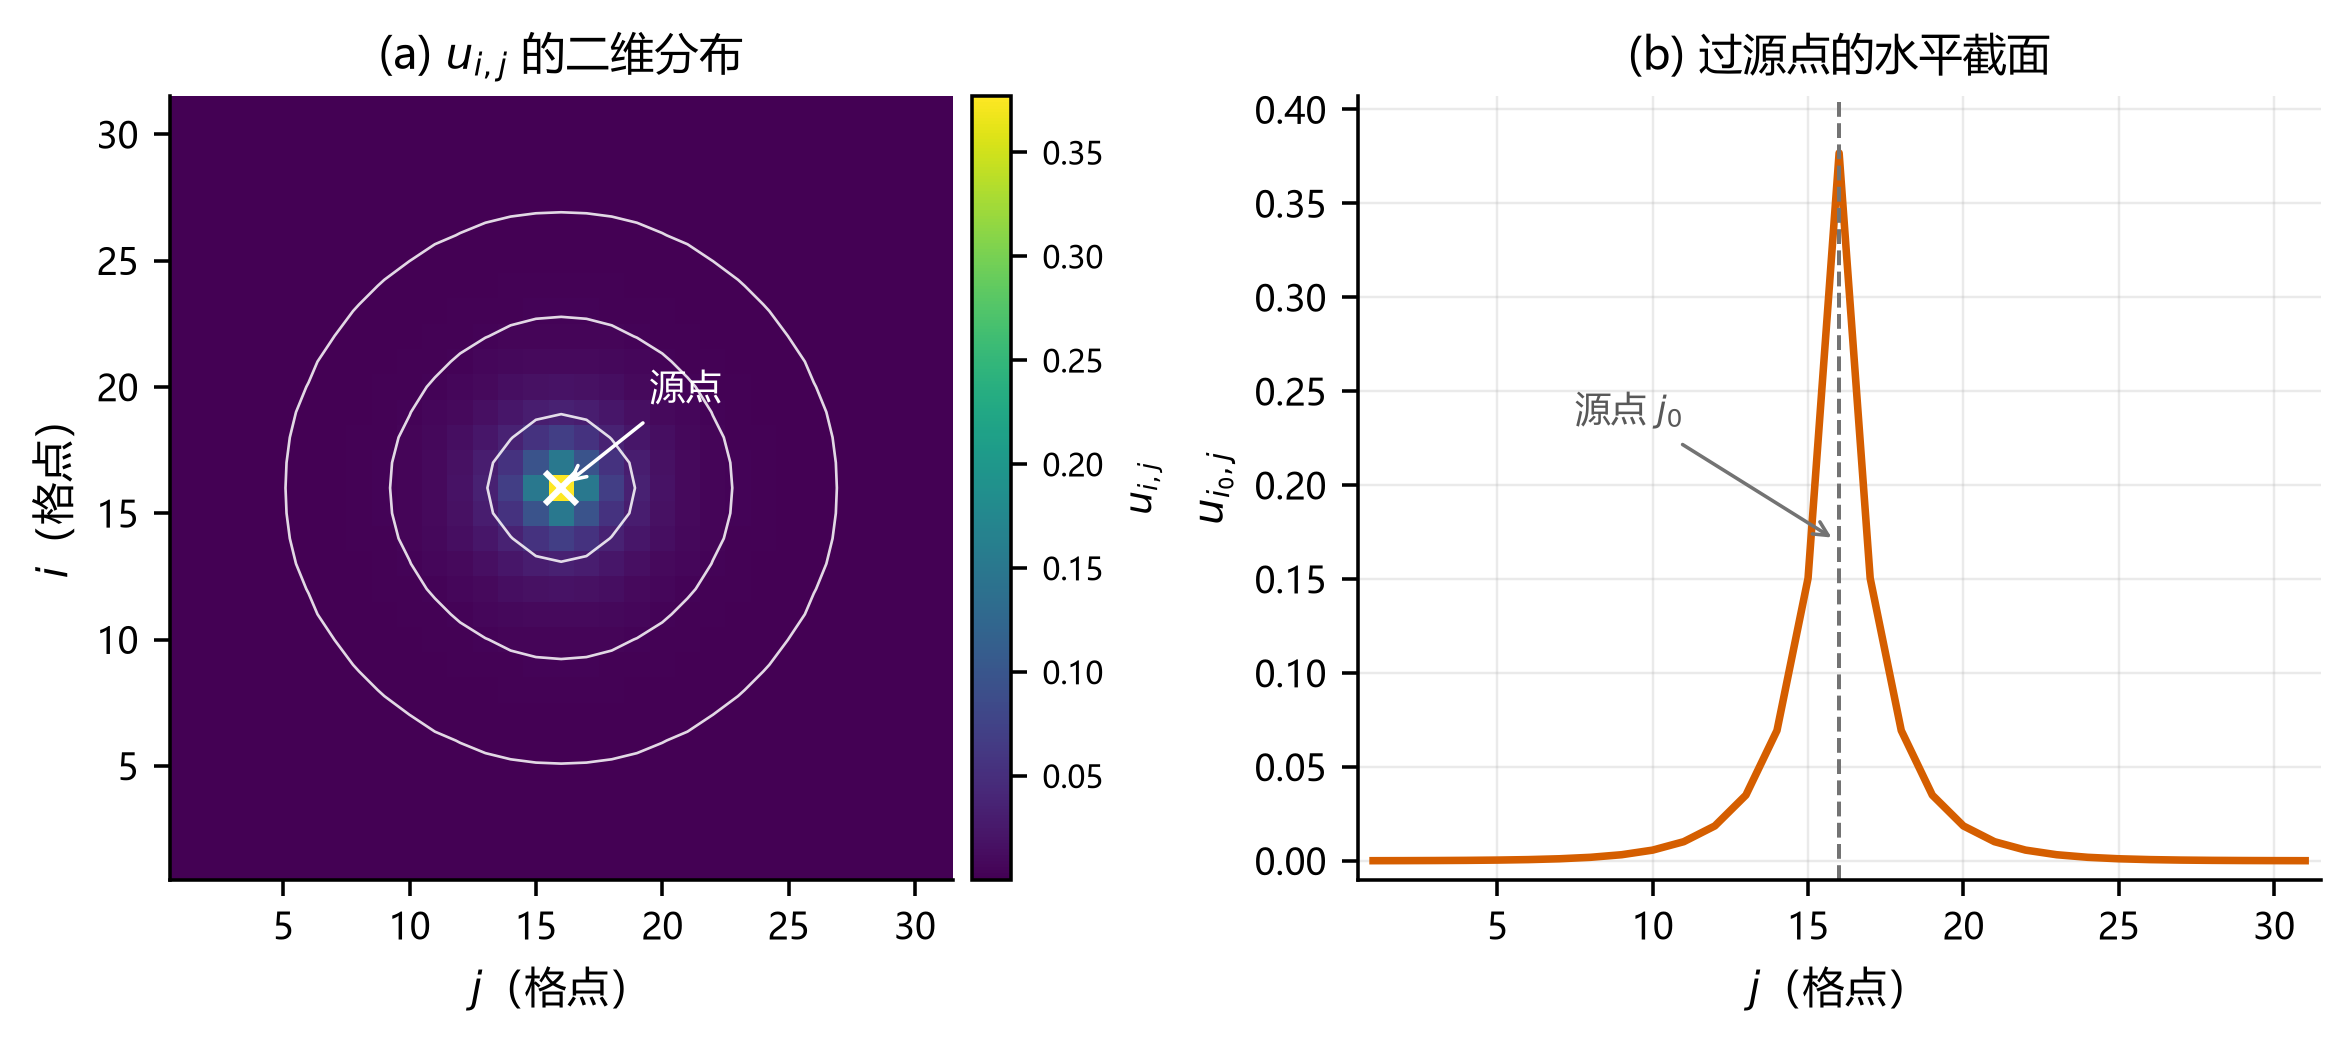
\includegraphics[width=0.72\linewidth]{../figures/fig1_task1.png}

\vfill

\begin{tabular}{rl}
\large 课程： & \large 计算物理 \\[0.45em]
\large 姓名： & \large \underline{\hspace{4.2cm}} \\[0.45em]
\large 学号： & \large \underline{\hspace{4.2cm}} \\[0.45em]
\large 专业： & \large \underline{\hspace{4.2cm}} \\[0.45em]
\large 日期： & \large 2026 年 11 月 \\
\end{tabular}

\vspace{1.2cm}
\end{titlepage}

% ===========================================================================
% 摘要
% ===========================================================================
\section*{摘\quad 要}
\addcontentsline{toc}{section}{摘要}

本文用逐点超松弛（SOR）迭代求解二维格点点源模型。模型在 $N\times N$ 个内部格点上离散
$-\nabla^2u+m^2u=s$，四周取零 Dirichlet 边界，中心格点放单位源，格距 $h=1$。我们实现了
字典序逐点 SOR，并用“按反对角线向量化”的等价写法加速；在 $N=31$、$m=0.5$、$\omega=1.5$
时，两种实现给出的扫描次数、残差和场值逐位相同。程序在 $N=7,9$ 的小网格上与稠密线性方程组
的直接解对照：阈值从 $10^{-4}$ 收紧到 $10^{-10}$ 时，最大解差由 $2.3\times10^{-5}$ 单调
降到 $1.1\times10^{-11}$，且始终低于 $\|A^{-1}\|_\infty\|r\|_\infty$ 的误差上界。

数值实验表明：$N=31$、$m=0.5$、$\omega=1.5$ 时响应最大值在源点
($u_{\max}=\UmaxTaskI$)，残差 $\RestaskI$，共 \KtaskI{} 次扫描；转置对称性达到机器精度。
固定 $N=63$，$m=0.2,0.5,1.0$ 的指数尾段衰减长度为 $\xi=\XiA,\XiB,\XiC$ 个格距，
$m\xi=\XiMA,\XiMB,\XiMC$ 近似为常数，支持 $\xi\propto1/m$；$N=127$ 的对照表明 $N=63$
对 $m\ge0.2$ 的中心区响应已足够准确。$\omega$ 扫描显示 $K(\omega)$ 在
$\omega\approx1.41$--$1.43$ 形成宽平台（$K=30$），比 Gauss--Seidel 的
$K_{\rm GS}=68$ 少 \RedThree；$\omega\to2$ 时收敛迅速变慢。三种 $m$ 下的经验最优
$\omega$ 为 $\WexpA,\WexpB,\WexpC$，均低于理论值
$\omega_{\rm th}=\WthA,\WthB,\WthC$。通过数值对角化验证谱半径公式，并收紧停止阈值
（$10^{-6}\to10^{-12}$）观察到经验最优由 $1.41$ 单调移向 $1.47$，说明这一偏差来自
有限阈值下的瞬态/前因子效应，而非公式或程序错误。

\vspace{0.8em}
\noindent\textbf{关键词：}格点点源模型；五点差分；逐点 SOR；谱半径；收敛因子；响应范围

\vspace{1.0em}
\noindent\rule{\linewidth}{0.4pt}

% ===========================================================================
\section{模型、离散方程与算法}
% ===========================================================================

\subsection{模型与离散化}

考虑二维正方形区域：内部有 $N\times N$ 个格点，四周再加一圈边界格点，格距取 $h=1$。
边界上的场固定为零，
\begin{equation}
u_{0,j}=u_{N+1,j}=u_{i,0}=u_{i,N+1}=0 .
\label{eq:bc}
\end{equation}
在中心格点 $(i_0,j_0)$ 放置单位点源，
\begin{equation}
s_{i,j}=\delta_{i,i_0}\,\delta_{j,j_0},
\qquad
i_0=j_0=\frac{N+1}{2}\quad(N\text{ 为奇数}).
\label{eq:source}
\end{equation}
模型方程为
\begin{equation}
-\nabla^2u+m^2u=s(x,y),
\qquad m>0 .
\label{eq:model}
\end{equation}
由于 $h=1$，$m$ 以格距为单位。用中心差分
$-\nabla_h^2u_{i,j}=4u_{i,j}-u_{i+1,j}-u_{i-1,j}-u_{i,j+1}-u_{i,j-1}$，得到
\begin{equation}
(4+m^2)u_{i,j}-u_{i+1,j}-u_{i-1,j}-u_{i,j+1}-u_{i,j-1}=s_{i,j}.
\label{eq:discrete}
\end{equation}
等价地，
\begin{equation}
u_{i,j}=\frac{s_{i,j}+u_{i+1,j}+u_{i-1,j}+u_{i,j+1}+u_{i,j-1}}{4+m^2}.
\label{eq:gsform}
\end{equation}

需要强调，\eqref{eq:model} 是一个带屏蔽质量项的标量方程，$u$ 是实数标量场，$m$ 是控制
响应衰减的参数；本文借用“在格点上求解方程、研究源产生的空间响应”的计算思想，
\textbf{不是格点 QCD 模拟}，不涉及规范场、夸克或量子场论。公式中的 $m$ 也不应解释为
某个粒子的物理质量。本文的指标均使用 1-based 编号；程序内部使用 0-based，二者只差 1。

矩阵 $A$ 对称正定，且为 M-矩阵，因此离散解存在唯一并满足最大值原理：当 $s\ge0$ 时
$u\ge0$，最大值在源点取得。这两条性质在后面用作程序正确性的辅助检查。

\subsection{逐点 SOR 更新}

按固定顺序扫描内部格点：$i$ 从 $1$ 到 $N$，$j$ 从 $1$ 到 $N$。对当前格点，先用
扫描过程中已经更新的邻点值计算 Gauss--Seidel 候选值
\begin{equation}
u_{i,j}^{\GS}
=\frac{s_{i,j}+u_{i+1,j}+u_{i-1,j}+u_{i,j+1}+u_{i,j-1}}{4+m^2},
\label{eq:gs}
\end{equation}
其中 $u_{i-1,j}$ 与 $u_{i,j-1}$ 是本轮已更新的值，$u_{i+1,j}$ 与 $u_{i,j+1}$ 仍是旧值。
再做 SOR 更新
\begin{equation}
u_{i,j}^{\rm new}=(1-\omega)u_{i,j}^{\rm old}+\omega\,u_{i,j}^{\GS},
\qquad 0<\omega<2 .
\label{eq:sor}
\end{equation}
$\omega=1$ 时退化为 Gauss--Seidel；$1<\omega<2$ 为超松弛。初始时所有内部格点取
$u_{i,j}=0$，每轮扫描后边界仍保持为零。

\subsection{残差与停止准则}

定义残差
\begin{equation}
r_{i,j}=s_{i,j}-\left[(4+m^2)u_{i,j}-u_{i+1,j}-u_{i-1,j}-u_{i,j+1}-u_{i,j-1}\right],
\qquad
\|r\|_\infty=\max_{1\le i,j\le N}|r_{i,j}| .
\label{eq:residual}
\end{equation}
每完成一次全格点扫描计算一次 $\|r\|_\infty$，当
\begin{equation}
\|r\|_\infty<10^{-6}
\label{eq:stop}
\end{equation}
时停止。程序同时设置最大扫描次数 $2\times10^{5}$；若达到上限仍未满足 \eqref{eq:stop}，
则报告“在最大迭代次数内未收敛”。本文所有正式实验均在阈值内收敛（表~\ref{tab:task3}
中所有点均满足 $\|r\|_\infty<10^{-6}$）。

\subsection{公平比较协议}

比较不同 $\omega$ 或不同 $m$ 时，除被研究的参数外，其余条件完全一致，见表~\ref{tab:protocol}。
这一协议是后文所有定量结论可比的前提。

\begin{table}[htbp]
\centering
\caption{数值实验的固定条件与变化量}
\label{tab:protocol}
\small
\begin{tabular}{p{3.2cm}p{10.6cm}}
\toprule
项目 & 设置 \\
\midrule
网格与边界 & 内部 $N\times N$ 个格点，外包一层零 Dirichlet 边界，格距 $h=1$ \\
源 & 中心格点，强度为 1，其余内部格点为 0 \\
初始场 & 所有内部格点 $u_{i,j}=0$ \\
扫描顺序 & $i$ 递增、$j$ 递增（字典序） \\
残差与停止 & 式~\eqref{eq:residual}；每轮扫描后检查 $\|r\|_\infty<10^{-6}$ \\
最大扫描次数 & $2\times10^{5}$ \\
变化量 & 任务 2、4 改变 $m$；任务 3、4 改变 $\omega$；其余量固定 \\
参考解 & 同一 $A$、$b$、边界下的稠密直接解（仅用于验证） \\
\bottomrule
\end{tabular}
\end{table}

\subsection{实现要点：反对角线与字典序的等价性}

逐点 SOR 本身是串行的，但可以按反对角线 $k=i+j$ 整条更新而不改变结果。理由如下：
对固定 $k$ 上的任一点 $(i,j)$，式~\eqref{eq:gs} 只用到 $(i-1,j)$、$(i,j-1)$（均在
$k-1$ 上）和 $(i+1,j)$、$(i,j+1)$（均在 $k+1$ 上），不依赖同一条对角线上的其他点。
因此把 $k$ 整条同时更新，与按任意顺序逐点更新同一条对角线，得到的数值完全相同。
按 $k=2,3,\ldots,2N$ 的顺序处理，就严格复现了 $i$ 外层、$j$ 内层的字典序扫描。

这一等价性把每轮扫描从“$N^2$ 次 Python 循环”变成“$2N$ 次向量化运算”，使 $N=63$ 的
大规模扫描成为可能；同时，我们保留了一份完全朴素的双层循环实现用于逐位核对。在
$N=31$、$m=0.5$、$\omega=1.5$ 时，两种实现的扫描次数同为 33，最终残差同为
$3.89\times10^{-7}$，全场最大差为 $0$（逐位相同），见第~\ref{sec:verify} 节。

% ===========================================================================
\section{程序实现与验证}
\label{sec:verify}
% ===========================================================================

\subsection{程序结构}

计算分为四层，均为确定性代码，不含随机数：
\begin{itemize}[leftmargin=2.1em,itemsep=0.15em,topsep=0.2em]
\item \texttt{code/sor2d.py}：网格与源项、残差、逐点 SOR（反对角线向量化）、朴素逐点
SOR、稠密矩阵与直接解、$\|A^{-1}\|_\infty$、$\rho_J$ 与 $\omega_{\rm th}$。
\item \texttt{code/experiments.py}：按第~\ref{tab:protocol} 节的协议运行任务 1--4 与
选做的理论对照，输出 \texttt{results/\allowbreak results.json} 与 \texttt{results/\allowbreak *.csv}。
\item \texttt{code/\allowbreak plot\_figures.py}：从 JSON 生成第~\ref{fig:task1}--\ref{fig:verify} 图。
\item \texttt{code/\allowbreak make\_report\_assets.py}：从 JSON 生成本文的 \texttt{numbers.tex} 与
各表格，保证正文数字与数据一致。
\end{itemize}
运行环境为 Python 3.14.7、NumPy 2.5.3、Matplotlib 3.11.2，全部使用 float64；
完整实验约 \Elapsed{} 秒。复现命令见附录~\ref{app:repro}。

\subsection{小网格直接解对照}

在 $N=7$ 与 $N=9$ 上，把内部未知量按行优先排列成 $N^2$ 维向量，构造
\begin{equation}
Au=b,\qquad
A=(4+m^2)I-S\otimes I-I\otimes S,
\label{eq:dense}
\end{equation}
其中 $S$ 是 $N\times N$ 的三对角矩阵，次对角元为 1；$b$ 是源项。用
\texttt{numpy.linalg.solve} 求直接解 $u^{\rm ref}$，再与同一离散方程、同一边界、
同一源项下的 SOR 解比较，定义
\begin{equation}
\epsilon_\infty=\max_{1\le i,j\le N}\left|u_{i,j}^{\SOR}-u_{i,j}^{\rm ref}\right|.
\label{eq:eps}
\end{equation}
由 $r=A(u^{\rm ref}-u^{\SOR})$ 可得误差上界
\begin{equation}
\epsilon_\infty\le\|A^{-1}\|_\infty\,\|r\|_\infty,
\qquad
\|A^{-1}\|_\infty=\max_{1\le i\le N^2}\sum_{j=1}^{N^2}|(A^{-1})_{ij}| .
\label{eq:bound}
\end{equation}

\begin{table}[htbp]
\centering
\caption{$N=7,9$、$m=0.5$、$\omega=1.5$ 时的直接解对照。$\epsilon_\infty$ 为 SOR 解与
直接解的最大差，最后一列为 $u-u^{\mathsf T}$ 的最大绝对非对称性。}
\label{tab:verify}
\footnotesize
\setlength{\tabcolsep}{4.2pt}
\begin{tabular}{cccccccc}
\toprule
$N$ & 阈值 & $K$ & $\|r\|_\infty$ & $\epsilon_\infty$ & $\epsilon_\infty/\|r\|_\infty$ & $\|A^{-1}\|_\infty$ & 非对称性 \\
\midrule
7 & $1\times10^{-4}$ & 14 & $6.97\times10^{-5}$ & $2.30\times10^{-5}$ & 0.33 & 2.409 & $3.5\times10^{-17}$ \\
7 & $1\times10^{-6}$ & 21 & $9.30\times10^{-7}$ & $2.55\times10^{-7}$ & 0.27 & 2.409 & $8.3\times10^{-17}$ \\
7 & $1\times10^{-8}$ & 28 & $4.55\times10^{-9}$ & $9.31\times10^{-10}$ & 0.20 & 2.409 & $5.6\times10^{-17}$ \\
7 & $1\times10^{-10}$ & 34 & $5.81\times10^{-11}$ & $2.87\times10^{-11}$ & 0.49 & 2.409 & $5.6\times10^{-17}$ \\
9 & $1\times10^{-4}$ & 15 & $4.98\times10^{-5}$ & $2.01\times10^{-5}$ & 0.40 & 2.941 & $4.2\times10^{-17}$ \\
9 & $1\times10^{-6}$ & 21 & $6.58\times10^{-7}$ & $2.87\times10^{-7}$ & 0.44 & 2.941 & $2.8\times10^{-17}$ \\
9 & $1\times10^{-8}$ & 29 & $9.94\times10^{-9}$ & $2.40\times10^{-9}$ & 0.24 & 2.941 & $4.2\times10^{-17}$ \\
9 & $1\times10^{-10}$ & 35 & $3.02\times10^{-11}$ & $1.09\times10^{-11}$ & 0.36 & 2.941 & $2.8\times10^{-17}$ \\
\bottomrule
\end{tabular}

\end{table}

表~\ref{tab:verify} 给出 8 组结果。可以看到：
\begin{itemize}[leftmargin=2.1em,itemsep=0.15em,topsep=0.2em]
\item 阈值从 $10^{-4}$ 收紧到 $10^{-10}$，$\epsilon_\infty$ 从 $2.30\times10^{-5}$
单调降到 $2.87\times10^{-11}$（$N=7$）和从 $2.01\times10^{-5}$ 降到
$1.09\times10^{-11}$（$N=9$），与阈值的收紧同步；
\item $\epsilon_\infty/\|r\|_\infty$ 在 $0.20$--$0.49$ 之间，均小于
$\|A^{-1}\|_\infty=2.409$（$N=7$）和 $2.941$（$N=9$），式~\eqref{eq:bound} 成立且偏保守；
\item 在阈值 $10^{-6}$ 处，$N=7$ 与 $N=9$ 的 $\epsilon_\infty$ 分别为
$2.55\times10^{-7}$ 与 $2.87\times10^{-7}$，比阈值本身还小约 3--4 倍。这说明
“残差小于 $10^{-6}$”并不等于“解误差等于 $10^{-6}$”：前者是后者的上界控制量，
实际误差取决于 $A^{-1}$ 和残差向量的结构；在 max 范数下，误差可以小于残差。
\end{itemize}

图~\ref{fig:verify} 把表~\ref{tab:verify} 画成双对数图。数据点与
$\epsilon_\infty=\|r\|_\infty$ 的虚线近似平行，说明在本题的阈值范围内误差与残差近似
成正比；点线 $\|A^{-1}\|_\infty\|r\|_\infty$ 始终位于数据点上方，验证了上界。

\begin{figure}[htbp]
\centering
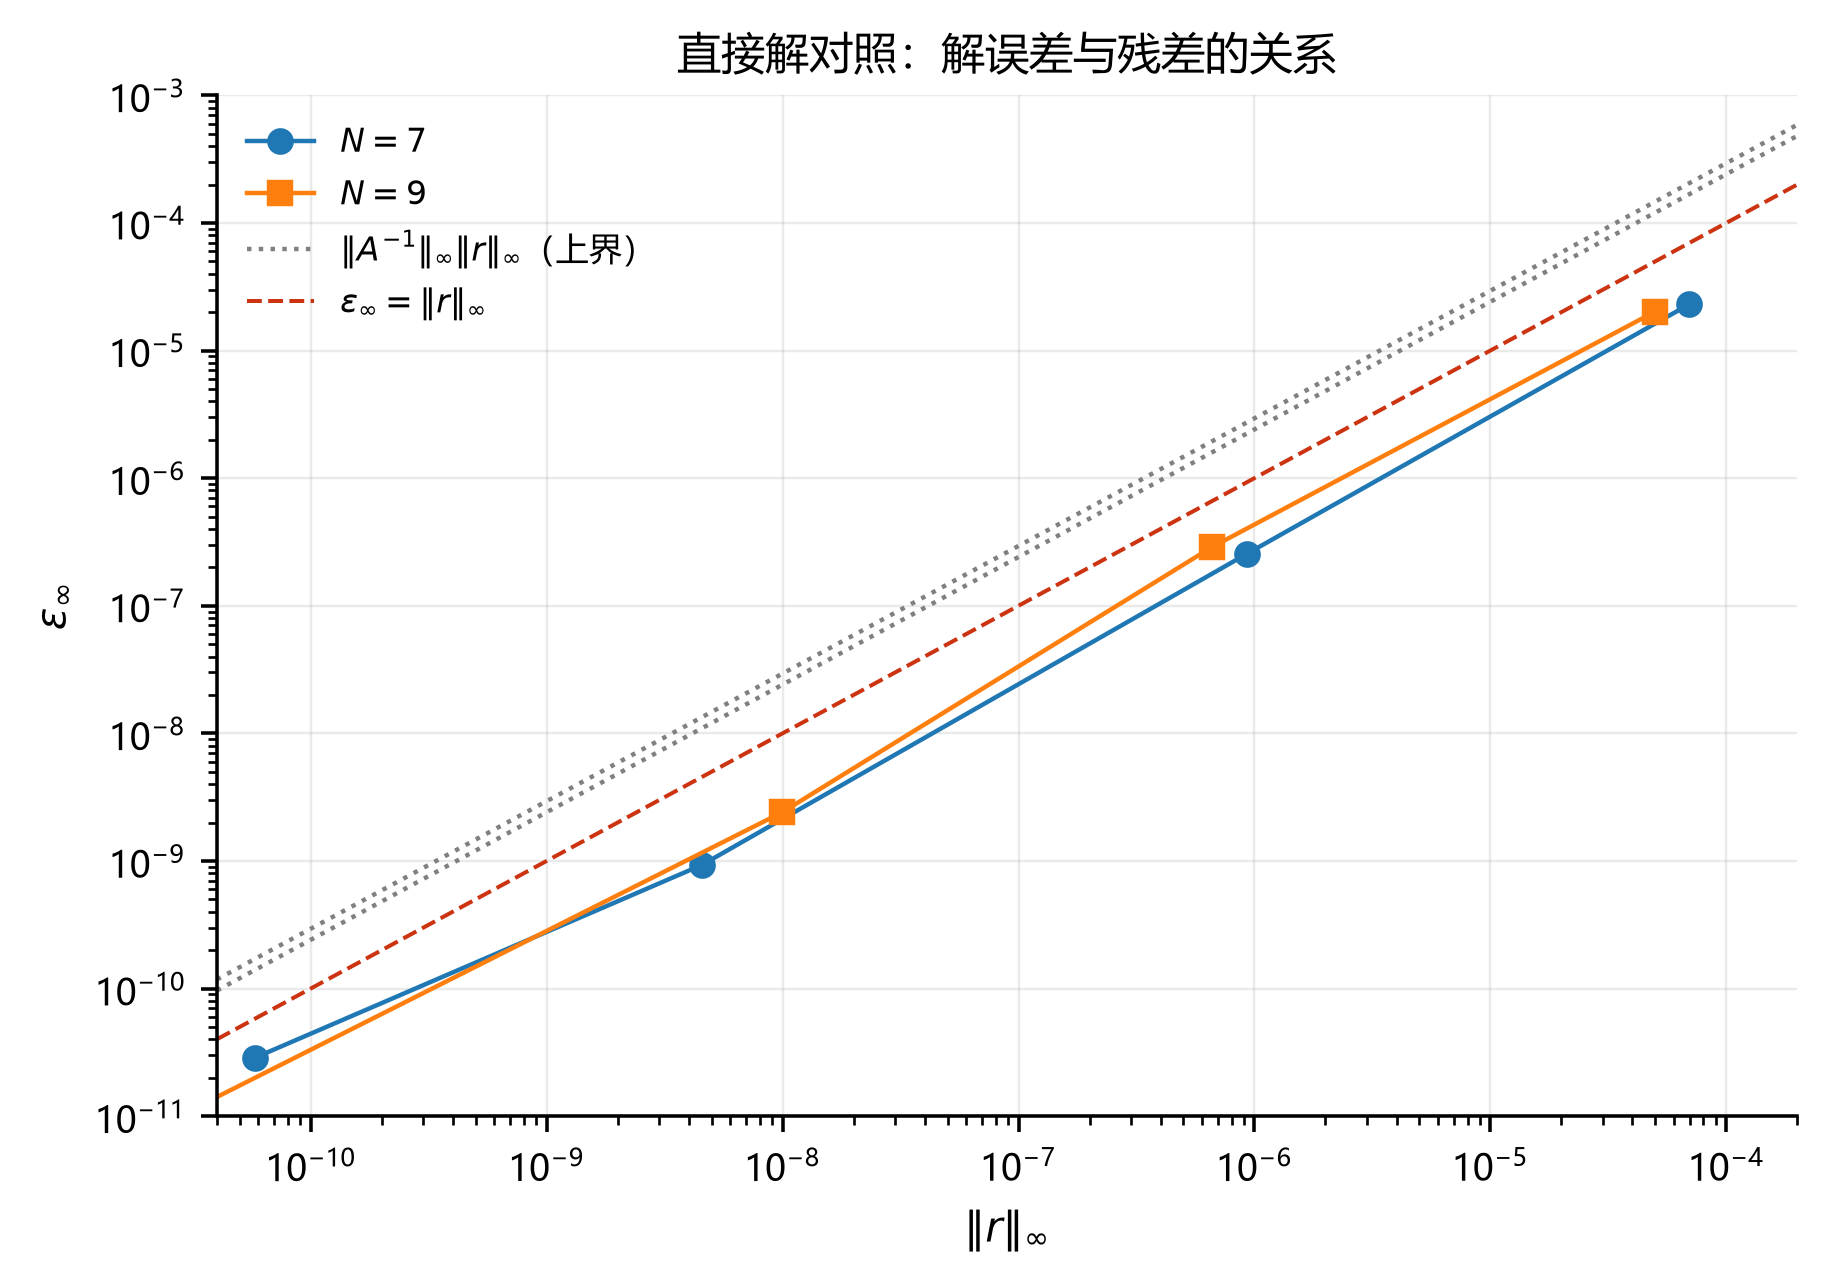
\includegraphics[width=0.70\linewidth]{../figures/fig6_verification.png}
\caption{小网格直接解对照：$\epsilon_\infty$ 随 $\|r\|_\infty$ 的变化。虚线为
$\epsilon_\infty=\|r\|_\infty$，点线为式~\eqref{eq:bound} 的上界
$\|A^{-1}\|_\infty\|r\|_\infty$。}
\label{fig:verify}
\end{figure}

\subsection{对称性、正性与实现一致性}

除直接解外，还做了三类检查：
\begin{enumerate}[leftmargin=2.1em,itemsep=0.15em,topsep=0.2em]
\item \textbf{转置对称性。} $N=7,9$ 时 $\max|u-u^{\mathsf T}|$ 为
$3\times10^{-17}$--$8\times10^{-17}$；任务 1 的 $N=31$ 解为 $2.8\times10^{-17}$，
达到双精度舍入水平。
\item \textbf{反射对称性。} 任务 1 的解关于源点的左右、上下反射的最大偏差为
$1.9\times10^{-7}$（相对 $u_{\max}$ 约 $5\times10^{-7}$）。它不是机器精度，而是与
停止阈值同量级的迭代误差：字典序扫描本身有方向性，收敛到有限残差时仍保留少量
方向性残差。这一量级与表~\ref{tab:verify} 中 $\epsilon_\infty$ 的量级一致，说明它不是
程序错误。
\item \textbf{正性。} 任务 1 的内部最小值为 $4.4\times10^{-7}>0$，与最大值原理一致。
\end{enumerate}
另外，反对角线实现与朴素逐点实现的结果逐位相同（最大差为 0），排除了向量化过程中
索引错位或更新顺序错误。上述检查与直接解对照一起，构成了本文对“程序正确”的独立证据；
仅凭热图“看起来合理”不足以说明问题。

% ===========================================================================
\section{任务 1：基准算例}
% ===========================================================================

取 $N=\Nmain$、$m=\Mmain$、$\omega=\Wmain$，按第~\ref{tab:protocol} 节的协议求解。
结果如图~\ref{fig:task1} 所示。

\begin{figure}[htbp]
\centering
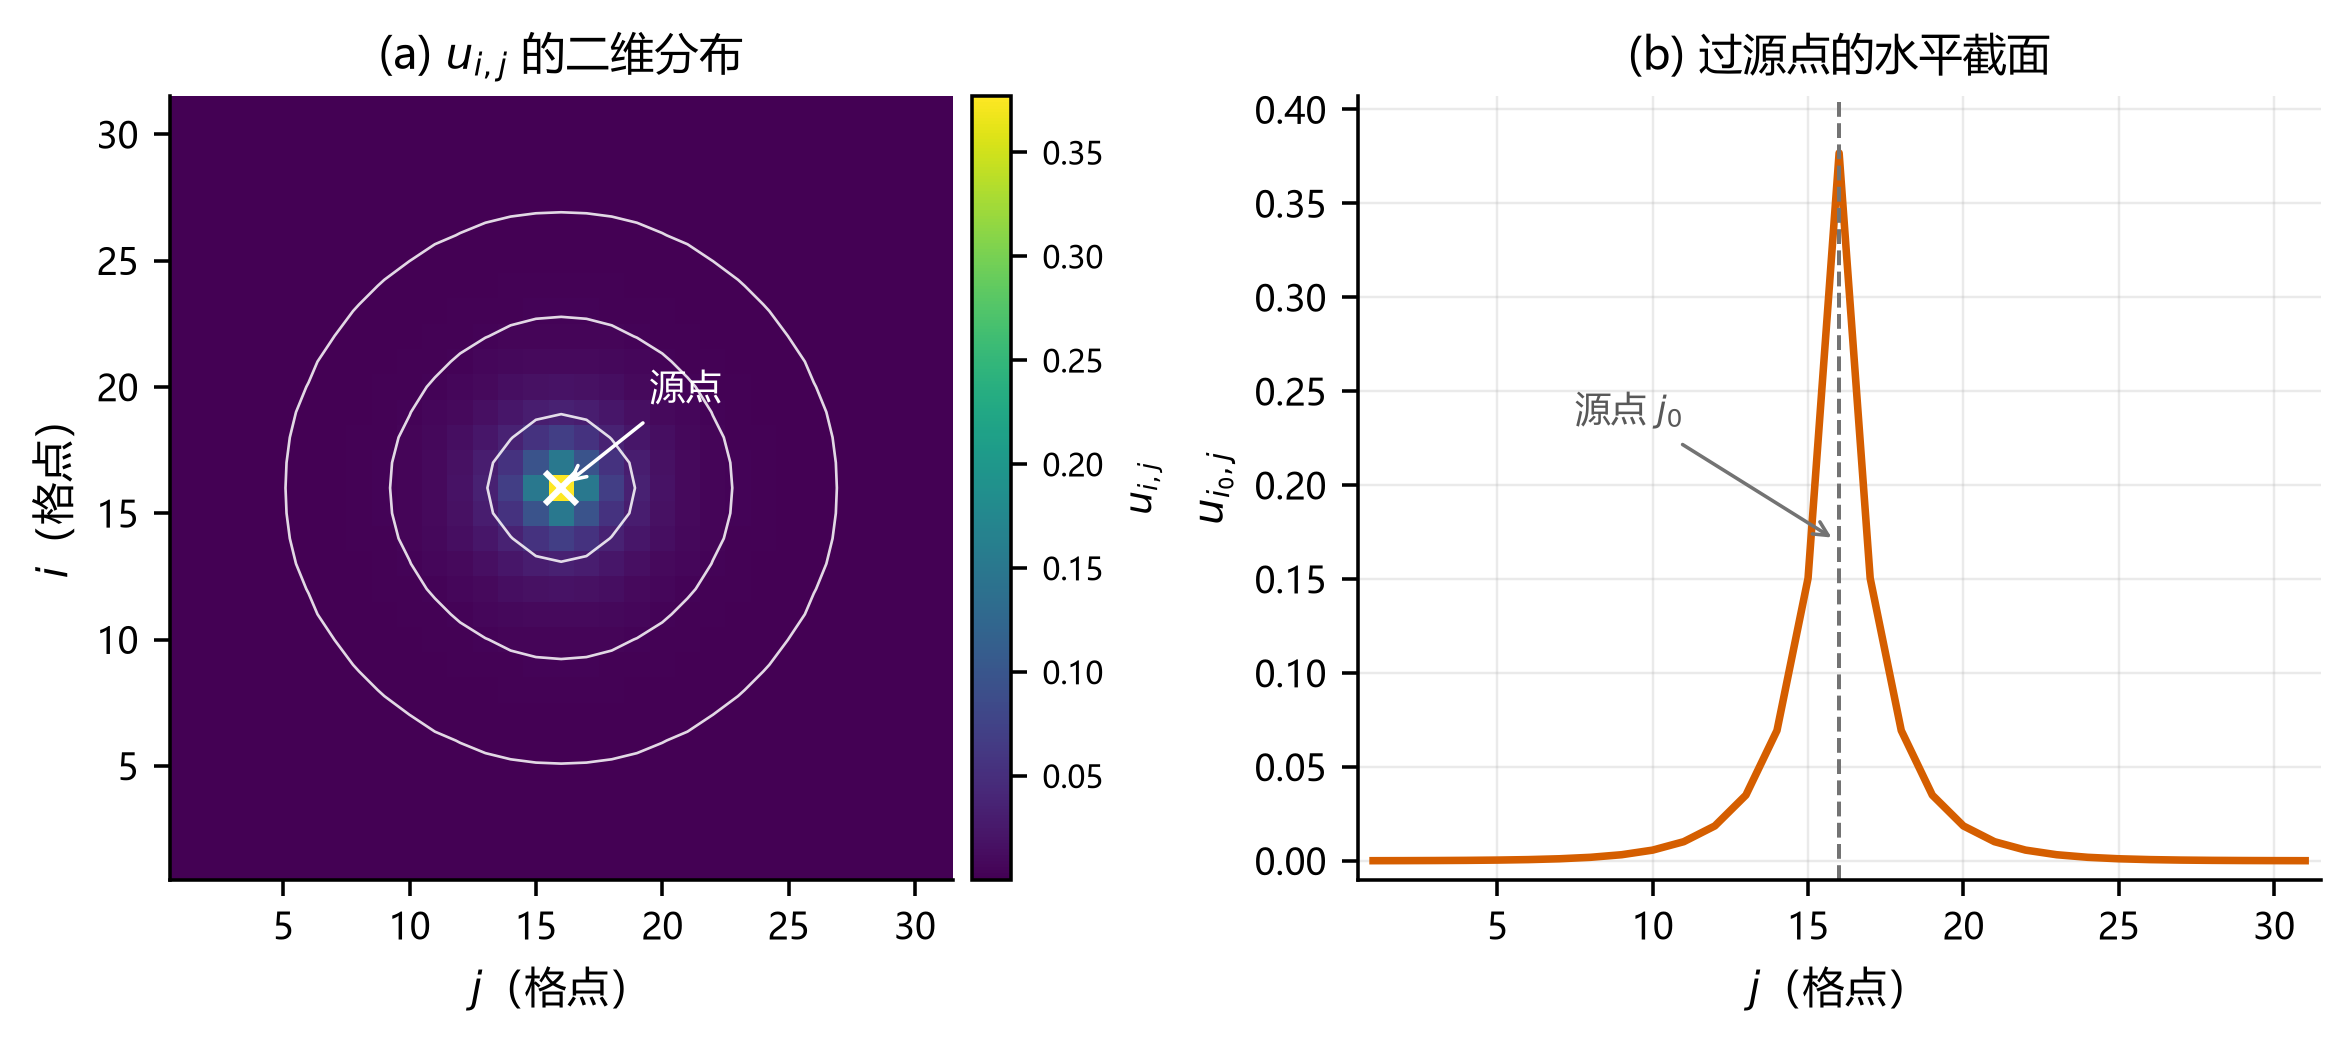
\includegraphics[width=\linewidth]{../figures/fig1_task1.png}
\caption{$N=31$、$m=0.5$、$\omega=1.5$ 的基准解。(a) $u_{i,j}$ 的二维分布，白色等值线
依次为最大值的 $10\%$、$1\%$、$0.1\%$，白色叉号标出源点；(b) 过源点的水平截面
$u_{i_0,j}$，竖直虚线为源点位置。}
\label{fig:task1}
\end{figure}

\paragraph{响应最大的位置。}
响应最大值出现在源点 $(16,16)$，$u_{\max}=\UmaxTaskI$。这与最大值原理一致：源项为正，
$A$ 为 M-矩阵，离散解非负且最大值在源点。图~\ref{fig:task1}(a) 中源点附近颜色最深，
等值线以源点为中心近似圆形，说明五点格式在 $h=1$ 的方形网格上基本各向同性；在
1--2 个格距内等值线略呈方形，这是离散拉普拉斯算子的各向异性。

\paragraph{离开源点后的变化。}
沿水平截面，响应从源点向外单调下降。源点与最近邻之间下降最快：$u_{i_0,j_0+1}/u_{\max}
=\RatioOne$，即一个格距内已损失约 60\%；之后进入近似指数衰减的尾段，$m=0.5$ 的
有效衰减长度约为 $1.74$ 个格距（第~\ref{sec:task2} 节）。图~\ref{fig:task1}(a) 的
$10\%$、$1\%$、$0.1\%$ 等值线半径依次增大，直观显示了“源点附近陡降、远处指数尾”的
结构。

\paragraph{对称性。}
解满足 $u_{i,j}=u_{j,i}$，转置非对称性为 $2.8\times10^{-17}$；关于源点的左右、上下
反射对称性在 $1.9\times10^{-7}$ 以内，与停止误差同量级（第~\ref{sec:verify} 节）。
内部最小值为 $4.4\times10^{-7}>0$，没有出现负值或棋盘振荡。

\paragraph{残差与迭代次数。}
最终 $\|r\|_\infty=\RestaskI<10^{-6}$，共扫描 $\KtaskI$ 次，未达到最大扫描次数。
该结果与朴素逐点实现逐位相同（第~\ref{sec:verify} 节）。若把 $\omega$ 改为 1.0，
$N=63$ 时需要 68 次（第~\ref{sec:task3} 节），说明 $\omega=1.5$ 已带来
明显加速；但 $\omega=1.5$ 并非 $N=63$ 时的最优值，第~\ref{sec:task3} 节会看到
$N=63$ 的经验最优在 $1.41$ 附近。

% ===========================================================================
\section{任务 2：\texorpdfstring{$m$}{m} 对响应范围的影响}
\label{sec:task2}
% ===========================================================================

固定 $N=63$、$\omega=1.5$，取 $m=0.2,0.5,1.0$，在同一张图上绘制过源点的归一化响应
$u_{i_0,j}/u_{i_0,j_0}$，如图~\ref{fig:task2}(a)。这里三个 $m$ 使用同一个 $\omega=1.5$，
是为了让比较只改变 $m$；收敛解本身与 $\omega$ 无关，$\omega$ 只影响达到阈值的扫描次数。

\begin{figure}[htbp]
\centering
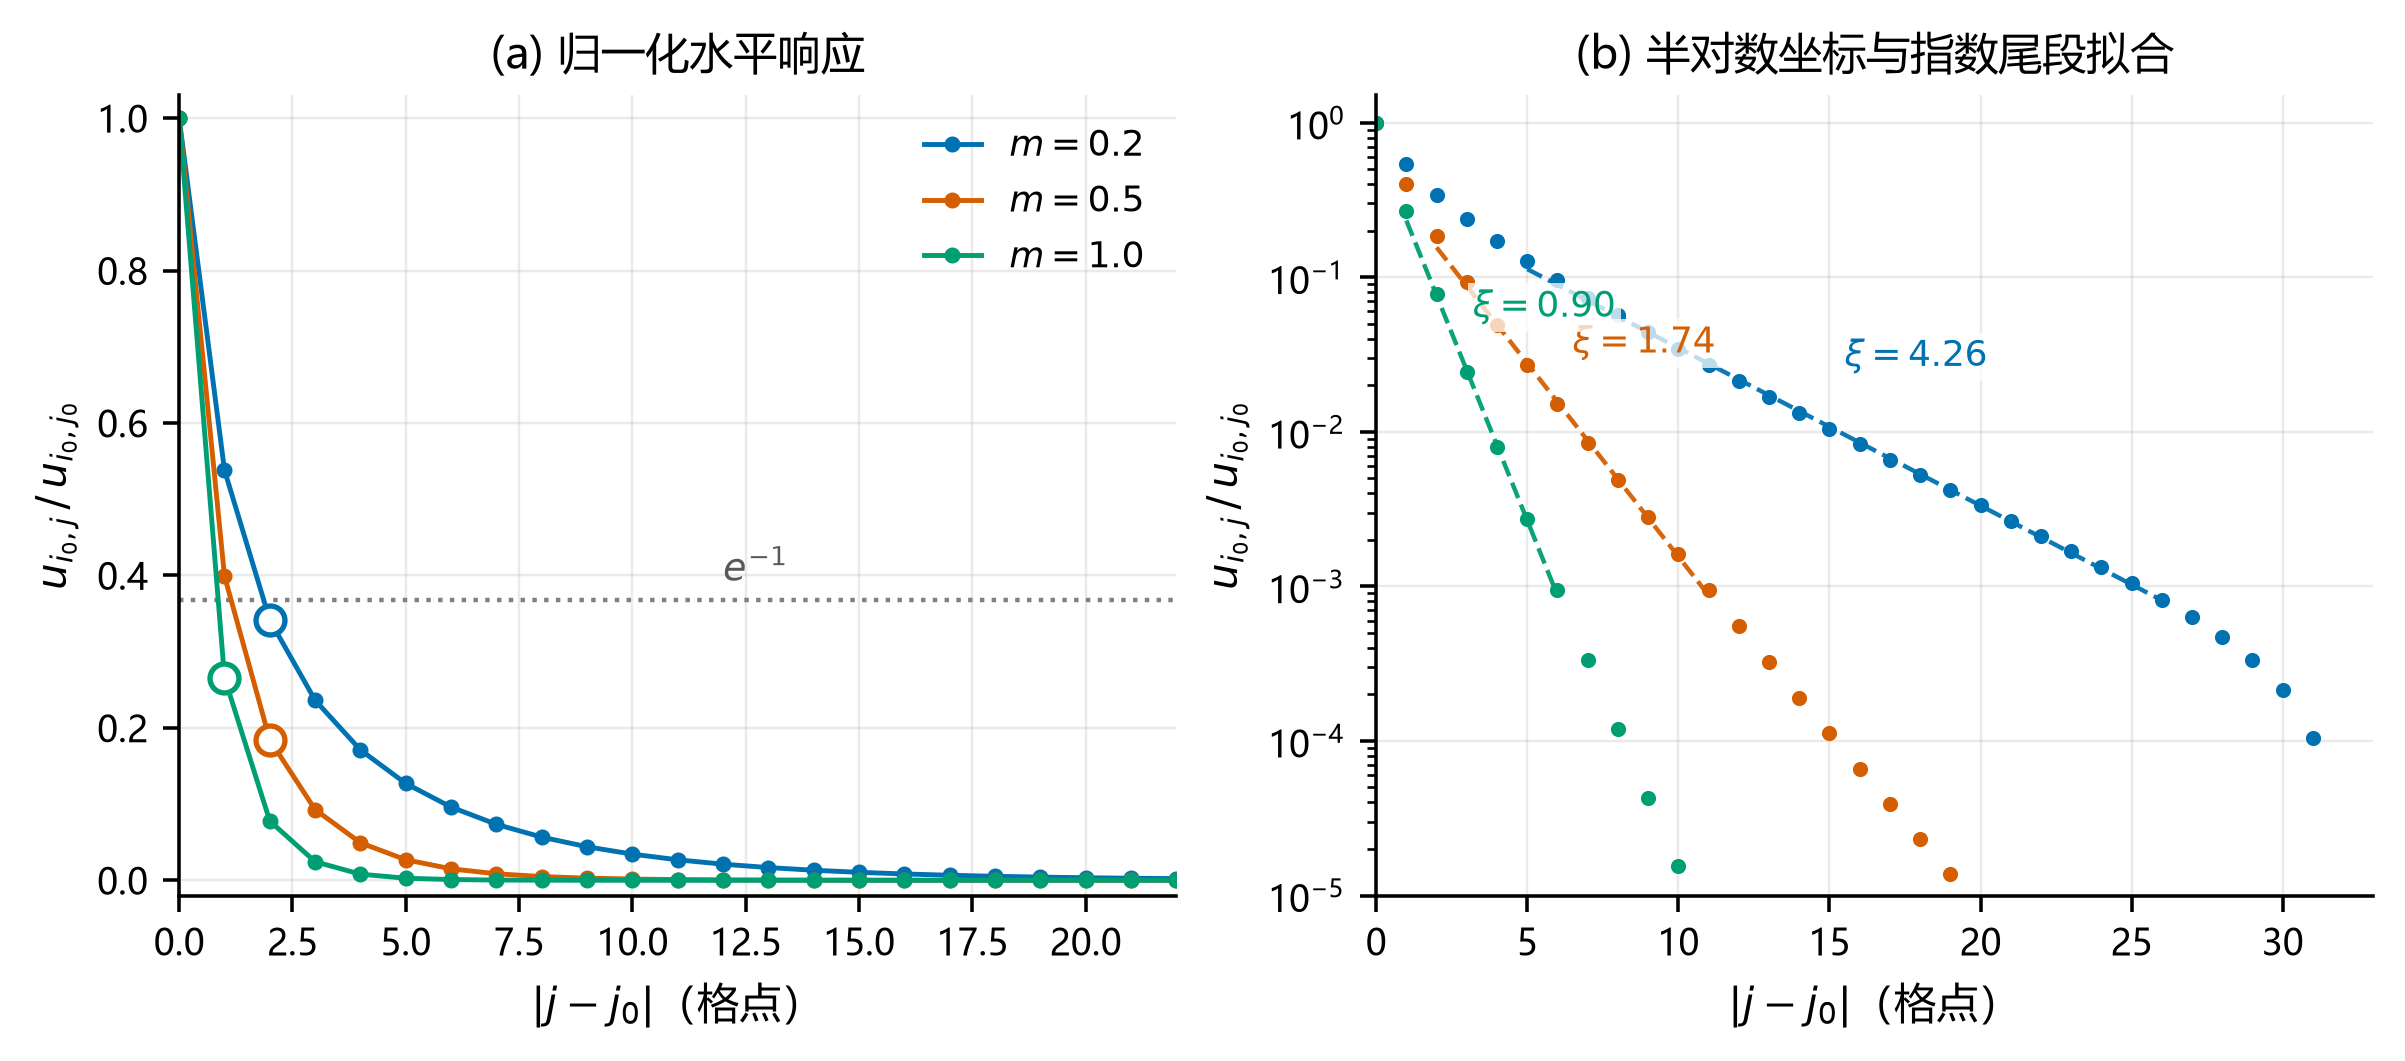
\includegraphics[width=\linewidth]{../figures/fig2_task2.png}
\caption{$N=63$ 时不同 $m$ 的归一化水平响应。(a) 线性坐标，空心圆标出首次降到
$e^{-1}$ 的格点；(b) 半对数坐标，虚线为 $10^{-1}\ge u/u_0\ge10^{-3}$ 尾段的指数拟合，
标注为有效衰减长度 $\xi$（单位：格距）。}
\label{fig:task2}
\end{figure}

\subsection{趋势}

$m$ 增大时，响应衰减明显加快，范围缩小。源点值本身也随 $m$ 增大而减小：
$u_{\max}=0.5297$、$0.3769$、$0.2540$（对应 $m=0.2$、$0.5$、$1.0$）。这与连续极限的直觉一致：
$m$ 越大，屏蔽越强，源的影响越局部化。归一化后，三条曲线在源点附近都从 1 开始，
但 $m=1.0$ 的曲线在 3--4 个格距内就降到 $10^{-2}$ 以下，而 $m=0.2$ 的曲线要到
15--16 个格距才降到同一水平。

\subsection{定量指标}

表~\ref{tab:task2} 给出三种指标。题目建议的“归一化响应首次降到 $e^{-1}$ 的距离”
$r_{1/e}$ 为 $2,2,1$，只在 1--2 个格距之间，远不如后两个指标敏感。原因是 $u_0$ 包含格点自能：源点与最近邻
之间本身就下降了 2.5--4 倍（$m=0.5$ 时 $u_1/u_0=0.399$，已接近 $e^{-1}=0.368$；
$m=1.0$ 时 $u_1/u_0=0.266<e^{-1}$；$m=0.2$ 时 $u_2/u_0\approx0.34<e^{-1}$）。
因此 $r_{1/e}$ 主要度量的是源点的格点自能，而不是尾部的衰减范围，不能区分 $m$。
这是一个值得说明的“指标陷阱”：题目允许自定义指标，我们保留 $r_{1/e}$ 作为对照，
同时采用两个更稳健的指标。

\begin{table}[htbp]
\centering
\caption{$N=63$ 时归一化响应的定量指标。$r_{1/e}$、$r_{1\%}$ 以格距为单位；
$\xi$ 为 $10^{-1}\ge u/u_0\ge10^{-3}$ 尾段 $\ln(u/u_0)$ 对距离的线性拟合斜率倒数，
拟合区间与 $R^2$ 一并给出。}
\label{tab:task2}
\footnotesize
\setlength{\tabcolsep}{4pt}
\begin{tabular}{ccccccccc}
\toprule
$m$ & $u_{\max}$ & $r_{1/e}$ & $r_{1\%}$ & $\xi$ & 拟合区间 & $R^2$ & $m\xi$ & $1/m$ \\
\midrule
$0.2$ & 0.5297 & 2 & 16 & 4.26 & 6--25 & 0.9996 & 0.85 & 5.00 \\
$0.5$ & 0.3769 & 2 & 7 & 1.74 & 3--10 & 0.9994 & 0.87 & 2.00 \\
$1.0$ & 0.2540 & 1 & 4 & 0.90 & 2--5 & 0.9997 & 0.90 & 1.00 \\
\bottomrule
\end{tabular}

\end{table}

第二个指标是响应降到源点值 $1\%$ 的距离 $r_{1\%}$：$m=0.2,0.5,1.0$ 分别为
$16,7,4$ 个格距，随 $m$ 增大而单调减小，比值约为 $2.3$ 与 $1.75$，与 $m$ 的比值
$2.5$ 与 $2$ 接近。第三个指标是尾段指数拟合得到的有效衰减长度 $\xi$：
$\xi=\XiA,\XiB,\XiC$，且 $m\xi=\XiMA,\XiMB,\XiMC$ 近似为常数，支持
\begin{equation}
\xi\simeq\frac{0.87}{m}.
\label{eq:xi}
\end{equation}
与连续的 $K_0(mr)$ 行为相比，$\xi$ 比 $1/m$ 低 $10\%$--$15\%$。原因有三：格点色散使
有效质量略大于 $m$；$K_0$ 还带有 $1/\sqrt{mr}$ 前因子，在对数斜率中贡献 $1/(2r)$；
拟合窗口有限（表~\ref{tab:task2} 中为 $k=6$--$25$、$3$--$10$、$2$--$5$）。
三个 $R^2$ 均大于 $0.999$，说明尾段确实近似指数。

\subsection{边界条件的影响}

零 Dirichlet 边界会压低远处的响应，从而可能缩短表观衰减长度。为定量评估，把区域扩大到
$N=127$（$h=1$ 不变，因此是扩大物理区域而非加密同一区域），比较同一 $m$ 下
$N=63$ 与 $N=127$ 的结果，见表~\ref{tab:boundary}。

\begin{table}[htbp]
\centering
\caption{边界条件影响：$N=63$ 与 $N=127$ 的对照。$\xi_{63}$、$\xi_{127}$ 使用相同的
拟合窗口；最后两列为两种网格上同一格点距离处 $u$ 的相对差（以 $N=127$ 的 $u_0$
归一）。}
\label{tab:boundary}
\small
\begin{tabular}{ccccc}
\toprule
$m$ & $\xi_{63}$ & $\xi_{127}$ & $\max_{k\le20}|\Delta u|/u_0$ & $\max_{k\le31}|\Delta u|/u_0$ \\
\midrule
$0.2$ & 4.257 & 4.284 & $1.68\times10^{-5}$ & $1.89\times10^{-4}$ \\
$0.5$ & 1.737 & 1.737 & $1.93\times10^{-11}$ & $5.15\times10^{-9}$ \\
$1.0$ & 0.896 & 0.896 & $4.60\times10^{-16}$ & $1.54\times10^{-15}$ \\
\bottomrule
\end{tabular}

\end{table}

$m=0.2$ 时，$\xi$ 从 $4.257$ 变为 $4.284$（差 $0.65\%$），中心区（$k\le20$）的最大
相对差为 $\BndA$，靠近边界处为 $\BndEdgeA$；$m=0.5$ 与 $m=1.0$ 的差分别只有
$1.9\times10^{-11}$ 与 $4.6\times10^{-16}$。这说明 $N=63$ 对 $m\ge0.2$ 的响应范围
已经足够；边界的影响按 $\exp[-N/(2\xi)]$ 估算，$m=0.2$ 时 $N/(2\xi)=7.4$，
$\exp(-7.4)\approx6\times10^{-4}$，与边界附近 $10^{-4}$ 量级的差一致。

因此，边界条件的方向是明确的：它只会让响应看起来衰减得更快，使测得的 $\xi$ 偏小；
若 $m$ 更小（$\xi$ 更大）或 $N$ 更小，这种偏差会变大，需要通过扩大 $N$、使用外推或
解析尾段修正来消除。本文的所有 $\xi$ 都是在 $N=63$ 下测得的有效值，而不是无限域
极限值；对 $m=0.2$ 应保留约 $1\%$ 的边界不确定度。

% ===========================================================================
\section{任务 3：松弛因子 \texorpdfstring{$\omega$}{omega} 的扫描}
\label{sec:task3}
% ===========================================================================

固定 $N=63$、$m=0.5$，按表~\ref{tab:protocol} 的统一协议扫描 $\omega$。先做粗扫
$\omega=1.0,1.1,\ldots,1.9,1.95$（11 个点），再在最小值附近做步长 $0.01$ 的细扫，
最后做步长 $0.002$ 的局部扫描。粗扫数据见表~\ref{tab:task3}，结果见图~\ref{fig:task3}。

\begin{table}[htbp]
\centering
\caption{$N=63$、$m=0.5$ 的粗扫结果。每个 $\omega$ 均从 $u=0$ 出发，按字典序 SOR
迭代到 $\|r\|_\infty<10^{-6}$，$K$ 为完整扫描次数。}
\label{tab:task3}
\small
\begin{tabular}{ccc}
\toprule
$\omega$ & $K$ & $\|r\|_\infty$ \\
\midrule
$1.00$ & 68 & $8.82\times10^{-7}$ \\
$1.10$ & 56 & $8.57\times10^{-7}$ \\
$1.20$ & 46 & $8.39\times10^{-7}$ \\
$1.30$ & 37 & $9.66\times10^{-7}$ \\
$1.40$ & 31 & $7.84\times10^{-7}$ \\
$1.50$ & 34 & $9.77\times10^{-7}$ \\
$1.60$ & 45 & $9.24\times10^{-7}$ \\
$1.70$ & 66 & $5.27\times10^{-7}$ \\
$1.80$ & 77 & $9.69\times10^{-7}$ \\
$1.90$ & 136 & $8.53\times10^{-7}$ \\
$1.95$ & 239 & $8.71\times10^{-7}$ \\
\bottomrule
\end{tabular}

\end{table}

\begin{figure}[htbp]
\centering
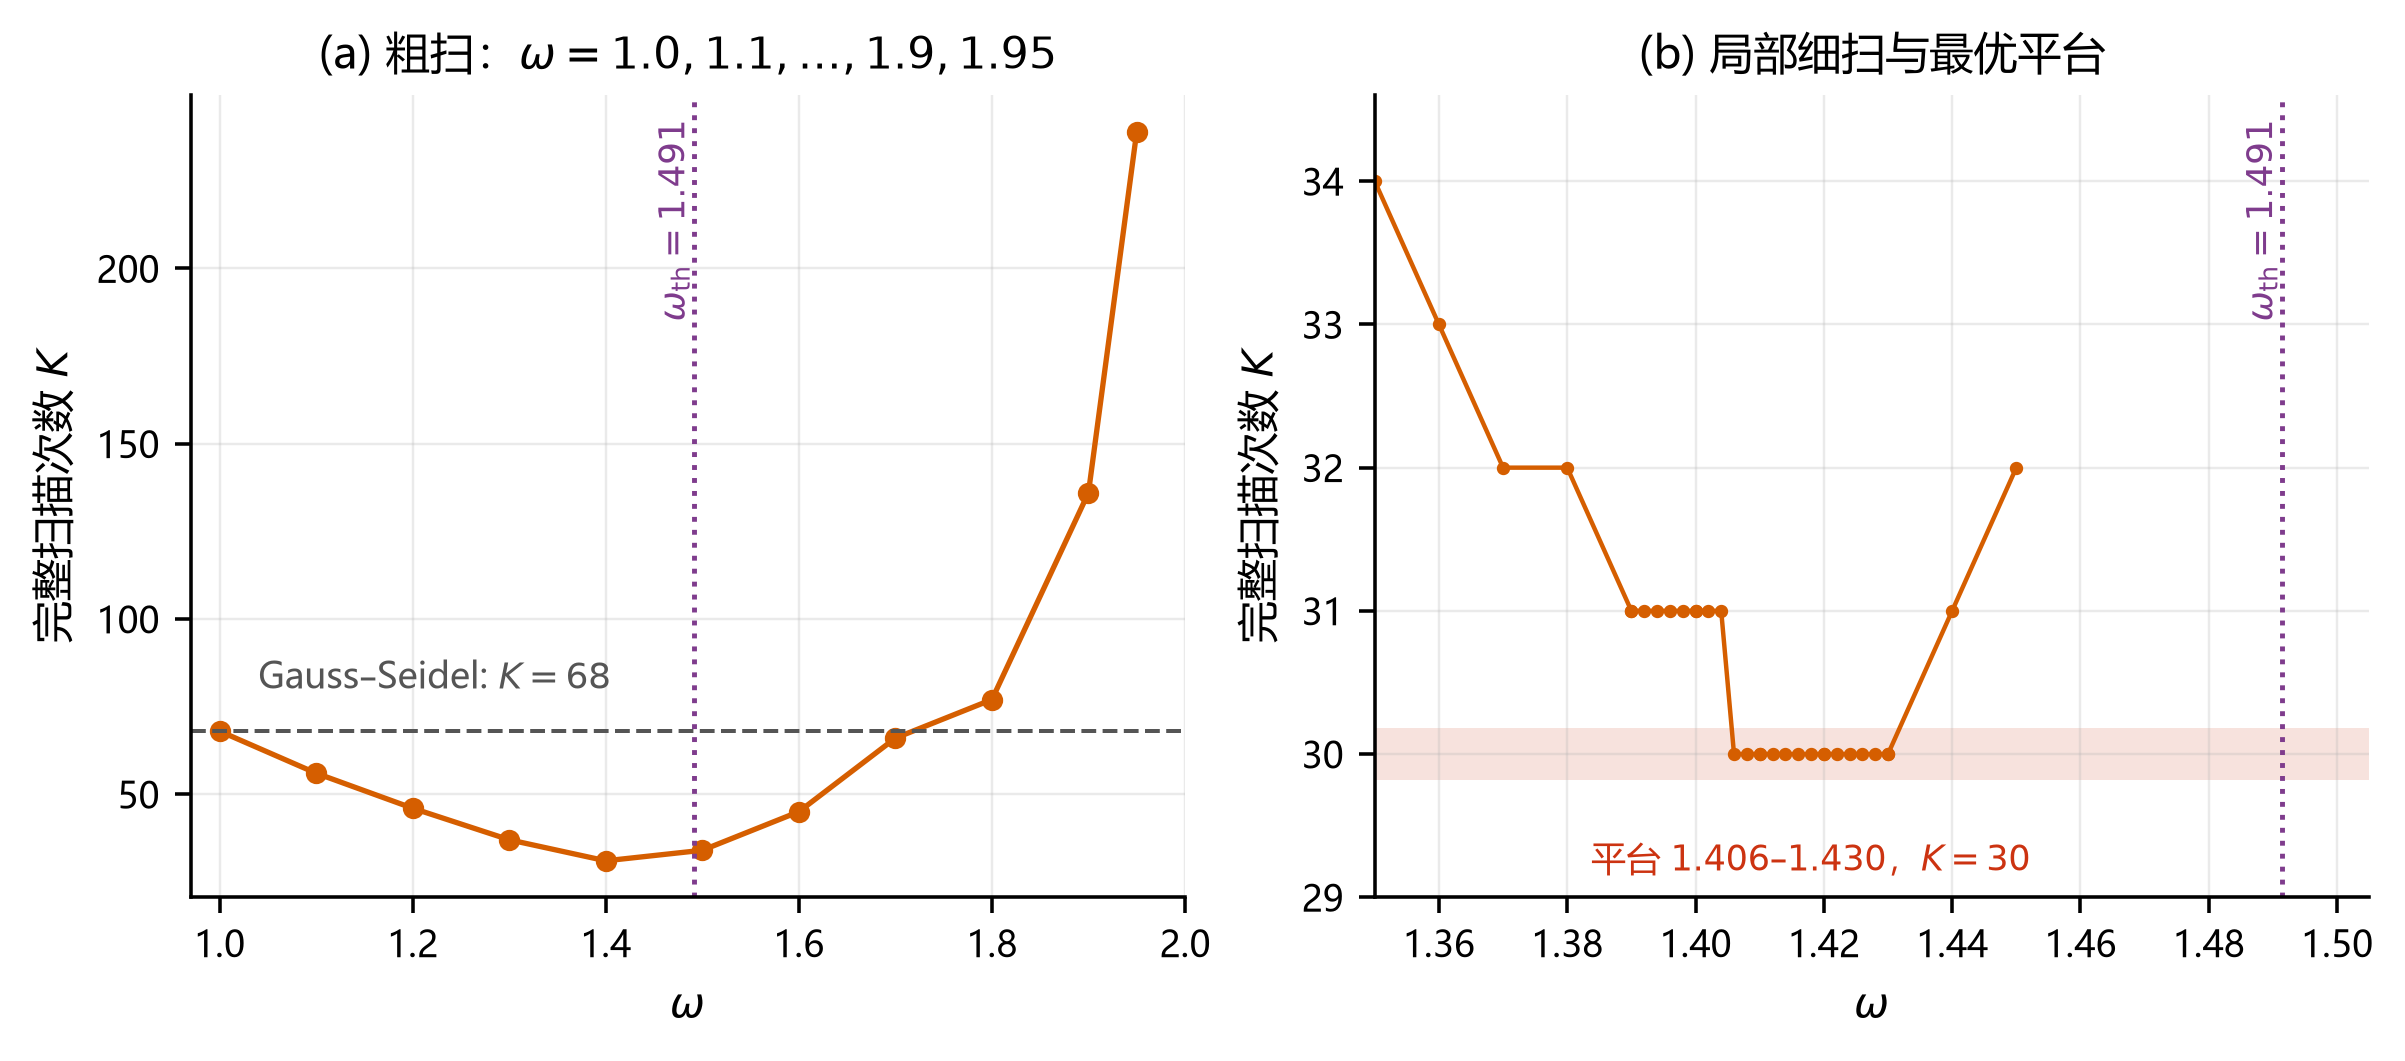
\includegraphics[width=\linewidth]{../figures/fig3_task3.png}
\caption{$N=63$、$m=0.5$ 时扫描次数随 $\omega$ 的变化。(a) 粗扫；水平虚线为
Gauss--Seidel（$\omega=1$）的 $K_{\rm GS}=68$，点线为理论值
$\omega_{\rm th}=1.491$。(b) 局部细扫与最优平台；阴影为 $K=30$ 的平台
$\omega=1.406$--$1.430$。}
\label{fig:task3}
\end{figure}

\subsection{结果}

粗扫的 $K(\omega)$ 呈明显的 U 形：$\omega=1.0$ 时 $K=68$，随后单调下降，
$\omega=1.4$ 时达到 $K=31$，之后回升；$\omega=1.5$ 为 34，$\omega=1.6$ 为 45，
$\omega=1.8$ 为 77，$\omega=1.9$ 为 136，$\omega=1.95$ 为 239。粗扫的最优点是
$\omega=\Wcoarse$（$K=\Kcoarse$）。

在粗扫最优点附近做步长 $0.01$ 的细扫（$1.35$--$1.45$），$K$ 在
$\omega=1.41,1.42,1.43$ 处均为 30；按“最小 $K$ 平台”的定义，细扫平台为
$1.41$--$1.43$，中点为 $1.42$。再做步长
$0.002$ 的局部扫描，得到 $K=30$ 的平台 $\omega=\PlatLo$--$\PlatHi$，平台中点为
$\PlatMid$。图~\ref{fig:task3}(b) 中的阴影即为该平台。

\subsection{三个问题的回答}

\paragraph{哪个范围收敛较快？}
$\omega\approx1.4$--$1.45$ 收敛最快；在 $10^{-6}$ 阈值下，最优平台为
$1.41$--$1.43$，平台中点约 $1.42$。$\omega=1.5$ 只比最优多 4 次扫描，说明最优点
附近相当平坦。

\paragraph{$\omega$ 接近 2 时收敛速度如何变化？}
迅速变慢，而且不是单调的“越大越好”。当 $\omega$ 超过理论最优值后，SOR 的谱半径为
$\rho_{\rm SOR}=\omega-1$（第~\ref{sec:theory} 节），于是
\begin{equation}
K\approx\frac{\ln(1/\epsilon)}{\ln[1/(\omega-1)]},
\qquad \omega>\omega_{\rm th}.
\label{eq:khigh}
\end{equation}
$\omega\to2$ 时分母趋于 0，$K$ 发散。数值上，$\omega=1.9$ 时 $K=136$，$\omega=1.95$
时 $K=239$，约为最优值的 4.5 倍与 8.0 倍；式~\eqref{eq:khigh} 给出的渐近估计分别为
131 与 269，前者与数值吻合，后者略高估（原因见第~\ref{sec:theory} 节）。因此实际使用
时应把 $\omega$ 选在最优平台内，而不是靠近 2。

\paragraph{与 Gauss--Seidel 相比减少了多少？}
Gauss--Seidel（$\omega=1$）需要 $K_{\rm GS}=68$ 次，最优 SOR 需要 30 次，减少
\RedThree，迭代次数比
\begin{equation}
S=\frac{K_{\rm GS}}{K_{\rm SOR}}=\Sthree .
\label{eq:s}
\end{equation}
这个加速是实在的，但远小于渐近理论预测的 $S_{\rm th}=\SthB$（第~\ref{sec:theory} 节）。
原因不是程序错误，而是 $10^{-6}$ 的阈值只覆盖了收敛过程的有限一段，渐近谱半径尚未
完全主导；这一点在第~\ref{sec:theory} 节用阈值扫描和谱半径核对进一步说明。

\paragraph{粗扫和细扫得到的最佳参数是否相同？为什么？}
不完全相同：粗扫为 $\Wcoarse$，细扫平台为 $1.41$--$1.43$（中点 $1.42$），相差
$0.01$--$0.02$，小于粗扫步长 $0.1$。原因有三：
(i) $K(\omega)$ 在最小值附近非常平坦，$K=30$ 的平台宽度约 $0.024$，而粗扫步长为
$0.1$，无法分辨平台内部的结构；
(ii) $K$ 是整数，平台内不同 $\omega$ 的 $K$ 只差 1--2 次，排序对舍入和阈值很敏感；
(iii) 停止阈值 $10^{-6}$ 使经验最优偏离渐近最优 $\omega_{\rm th}=1.491$（见
第~\ref{sec:theory} 节），因此“最优”本身是阈值相关的。
更稳健的表述是：在 $10^{-6}$ 阈值下，最优平台为 $\PlatLo$--$\PlatHi$，而不是某一个
精确的 $\omega$。粗扫与细扫的结果在此平台内一致。

% ===========================================================================
\section{任务 4：\texorpdfstring{$m$}{m} 对最优 \texorpdfstring{$\omega$}{omega} 的影响}
\label{sec:task4}
% ===========================================================================

对 $m=0.2,0.5,1.0$ 重复任务 3 的流程：步长 $0.05$ 的粗扫、最优点附近步长 $0.01$ 的
细扫、步长 $0.001$ 的局部扫描。结果见表~\ref{tab:task4} 与图~\ref{fig:task4}。
表中“实验最优 $\omega$”取最小 $K$ 平台的中点；平台范围一并列出，以避免把平台内的
任意一点误认为精确最优。

\begin{table}[H]
\centering
\caption{$N=63$ 时不同 $m$ 的最优 $\omega$、对应迭代次数、Gauss--Seidel 迭代次数与
迭代次数比 $S$。理论值 $\omega_{\rm th}$ 由式~\eqref{eq:wth} 给出。}
\label{tab:task4}
\small
\setlength{\tabcolsep}{4.5pt}
\begin{tabular}{ccccccc}
\toprule
$m$ & 实验最优 $\omega$ & $K_{\rm SOR}$ & $K_{\rm GS}$ & $S=K_{\rm GS}/K_{\rm SOR}$ & 理论 $\omega_{\rm th}$ & 最优平台 \\
\midrule
$0.2$ & 1.684 & 63 & 316 & 5.02 & 1.7413 & 1.681--1.687 \\
$0.5$ & 1.418 & 30 & 68 & 2.27 & 1.4914 & 1.405--1.430 \\
$1.0$ & 1.174 & 17 & 23 & 1.35 & 1.2490 & 1.158--1.190 \\
\bottomrule
\end{tabular}

\end{table}

\begin{figure}[H]
\centering
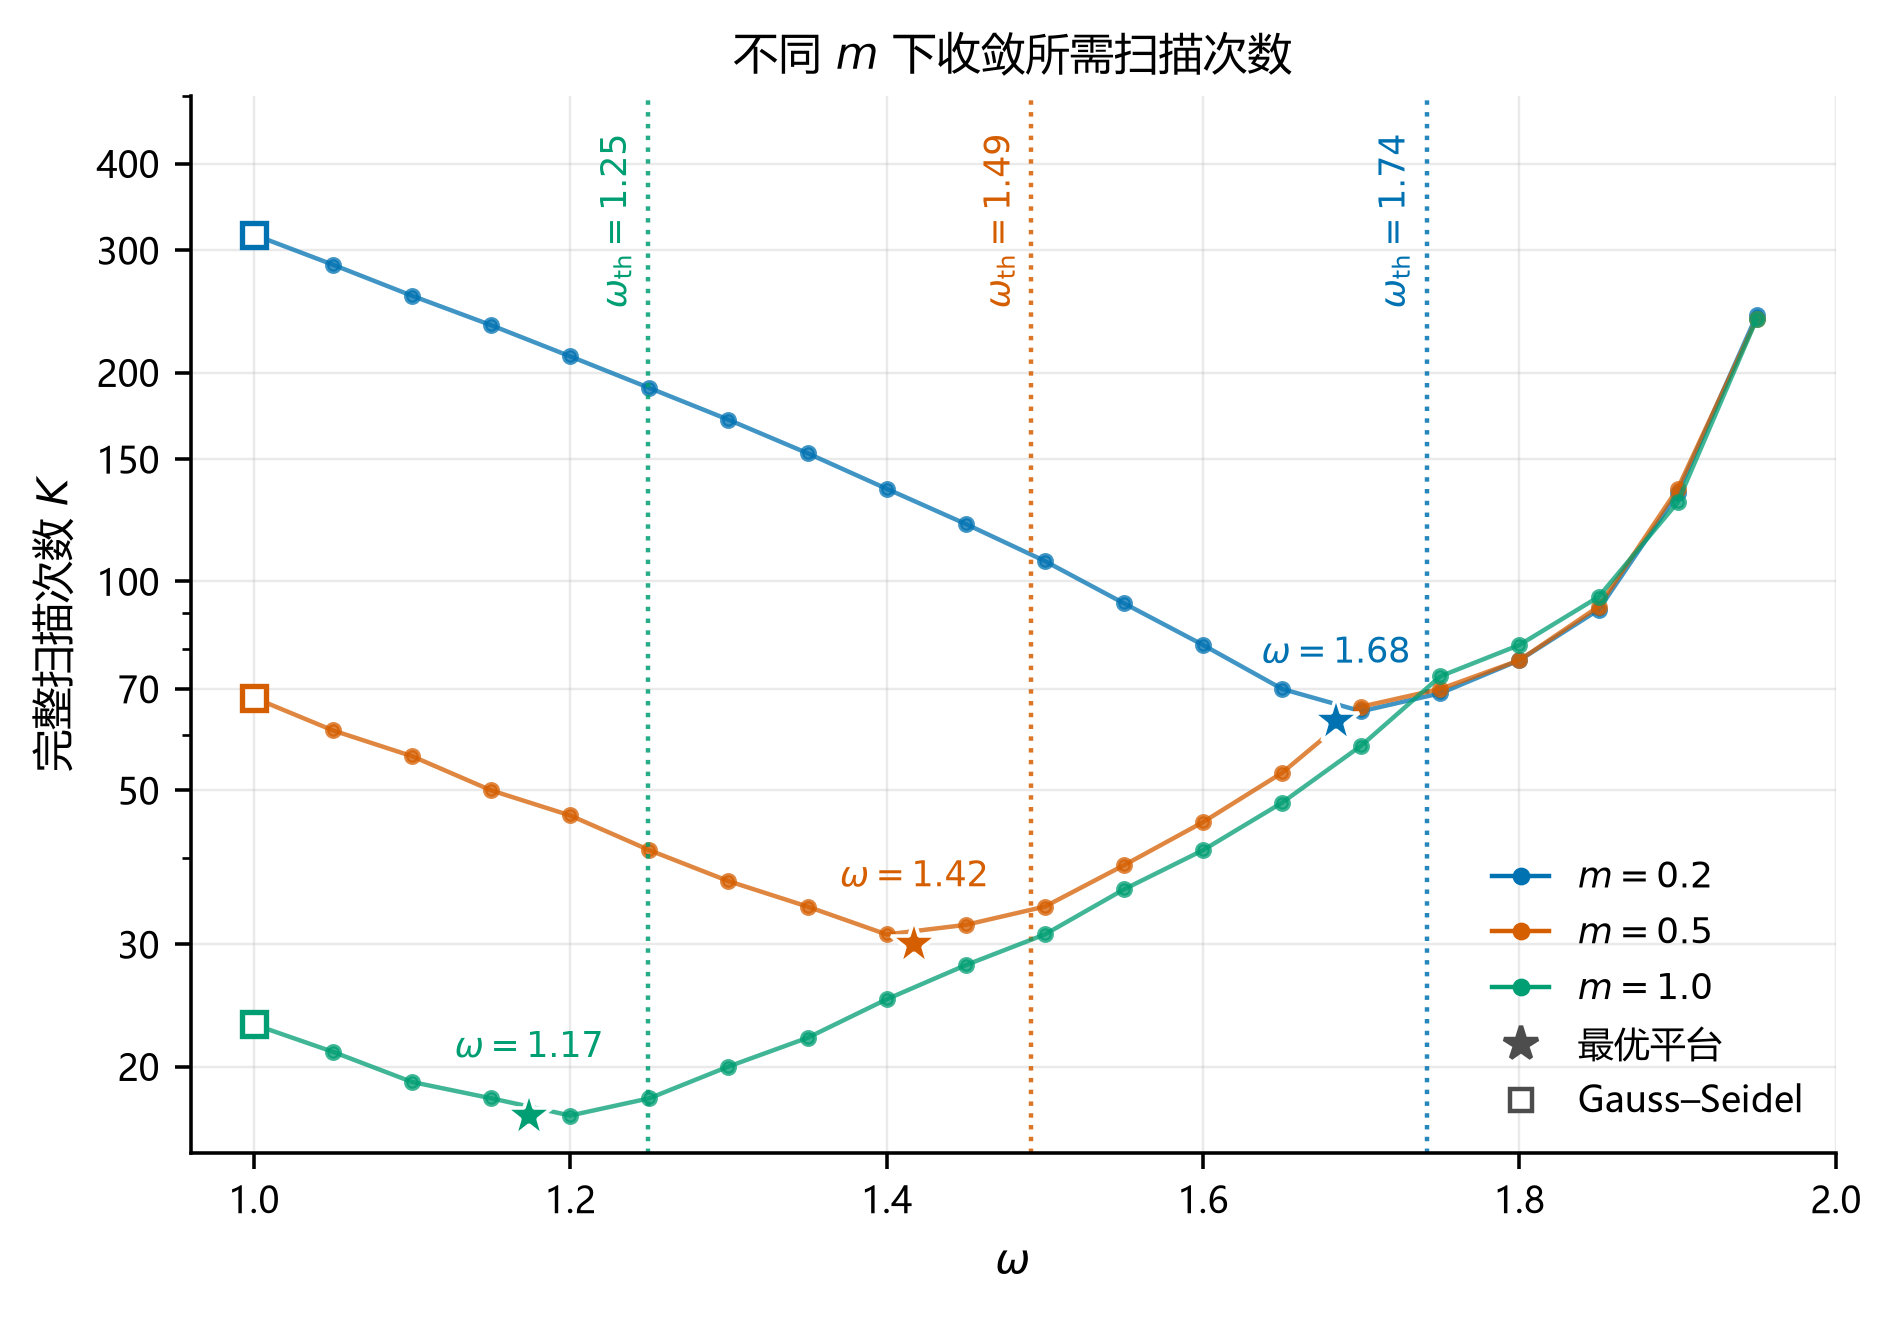
\includegraphics[width=\linewidth]{../figures/fig4_task4.png}
\caption{三种 $m$ 下 $K(\omega)$ 随 $\omega$ 的变化（对数纵轴）。星号为最优平台中点，
空心方块为 Gauss--Seidel，点线为理论 $\omega_{\rm th}$。}
\label{fig:task4}
\end{figure}

\subsection{趋势}

$m$ 减小时，最优 $\omega$ 增大：$\WexpA\to\WexpB\to\WexpC$（$m=0.2\to0.5\to1.0$），
理论值也按同一方向变化：$\WthA\to\WthB\to\WthC$。原因是 $m$ 越小，Jacobi 谱半径
$\rho_J=4\cos[\pi/(N+1)]/(4+m^2)$ 越接近 1，问题越病态，需要更强的超松弛来加速
低频模；$\omega_{\rm th}=2/(1+\sqrt{1-\rho_J^2})$ 随 $\rho_J\to1$ 单调增大并趋于 2。

迭代次数比 $S$ 随 $m$ 增大而减小：$S=\SA,\SB,\SC$。这看似与“$m$ 越小越难”一致，
但更准确的解释是：$m$ 大时问题本身很容易，Gauss--Seidel 也只需 $K_{\rm GS}=23$ 次
（$m=1.0$），SOR 能节省的绝对次数有限，$S$ 自然小；$m=0.2$ 时
$K_{\rm GS}=316$，SOR 只需 63 次，$S$ 达到 5.02。换句话说，$S$ 同时度量了问题的
难度和 SOR 的相对收益，不能单独作为“SOR 好不好”的绝对指标。

另一个值得注意的现象是：$\omega=1.95$ 时三种 $m$ 的 $K$ 几乎相同（约 239--242），
而 $\omega=1.0$ 时 $K$ 从 316 变到 23。这与式~\eqref{eq:khigh} 一致：高 $\omega$
分支的谱半径 $\rho_{\rm SOR}=\omega-1$ 与 $m$ 无关，所以迭代次数也几乎与 $m$ 无关；
$m$ 的影响主要体现在低 $\omega$ 分支和最优 $\omega$ 的位置上。

\subsection{经验最优与理论值的差异}

三种 $m$ 下经验最优都低于理论值，差 $\Delta\omega=0.057,0.073,0.075$。这一差异
不是程序错误：谱半径的数值对角化与公式逐点吻合（表~\ref{tab:rho}），直接解对照也
通过（表~\ref{tab:verify}）。差异来自“有限阈值 + 瞬态”：
\begin{itemize}[leftmargin=2.1em,itemsep=0.15em,topsep=0.2em]
\item 理论 $\omega_{\rm th}$ 最小化的是\emph{渐近}谱半径；实际停止在
$\|r\|_\infty=10^{-6}$，只经历了约 6 个量级的下降，迭代尚未完全进入由最慢模主导的
渐近阶段。
\item 初值是 $\delta$ 源，包含所有模式。Gauss--Seidel 在最初几步快速压低高频，
使其实际 $K$ 小于渐近估计；SOR 在 $\omega_{\rm th}$ 附近迭代矩阵接近亏损、非正态性
强，瞬态可持续数十步，使其实际 $K$ 大于渐近估计。
\item 两种效应叠加，使 $K(\omega)$ 的极小点偏向较小的 $\omega$；阈值越松，这种偏移
越明显。
\end{itemize}
第~\ref{sec:theory} 节用“阈值扫描”直接验证了这一点：把阈值从 $10^{-6}$ 收紧到
$10^{-12}$，经验最优从 $1.41$ 单调移到 $1.47$，逐步逼近 $\omega_{\rm th}=1.491$。

\subsection{扫描间隔与停止阈值的影响}

表~\ref{tab:task4} 中的平台宽度差异很大：$m=0.2$ 为 $1.681$--$1.687$（宽 $0.006$），
$m=0.5$ 为 $1.405$--$1.430$（宽 $0.025$），$m=1.0$ 为 $1.158$--$1.190$（宽 $0.032$）。
平台越宽，$K$ 对 $\omega$ 越不敏感，“最优 $\omega$”的确定就越依赖于扫描间隔。
若用步长 $0.1$ 的粗扫，$m=0.5$ 会得到 $1.4$；用步长 $0.01$ 会得到 $1.41$--$1.43$ 的平台；二者
都落在平台内，差别不表示哪一个“错”。因此本文报告平台和中点，而不是过度解读最后一位
小数。

阈值的影响更系统：表~\ref{tab:threshold} 给出同一 $m=0.5$ 下四个阈值的扫描结果。
阈值每收紧两个量级，$K_{\rm SOR}$ 与 $K_{\rm GS}$ 都增加，但 $K_{\rm SOR}$ 增加得
较慢，$S$ 从 $2.27$ 升到 $2.72$；经验最优 $\omega$ 从 $1.41$ 移到 $1.47$。这说明
“SOR 比 GS 快多少”以及“最优 $\omega$ 是多少”都不是与阈值无关的常数；报告数值时
必须同时给出阈值。

\begin{table}[htbp]
\centering
\caption{$N=63$、$m=0.5$ 时停止阈值对经验最优 $\omega$ 与迭代次数比的影响。
每个阈值下都在 $\omega=1.30$--$1.55$ 内以步长 $0.01$ 扫描。}
\label{tab:threshold}
\small
\begin{tabular}{ccccc}
\toprule
阈值 $\epsilon$ & 经验最优 $\omega$ & $K_{\rm SOR}$ & $K_{\rm GS}$ & $S$ \\
\midrule
$1\times10^{-6}$ & $1.41$ & 30 & 68 & 2.27 \\
$1\times10^{-8}$ & $1.44$ & 42 & 103 & 2.45 \\
$1\times10^{-10}$ & $1.45$ & 55 & 140 & 2.55 \\
$1\times10^{-12}$ & $1.47$ & 65 & 177 & 2.72 \\
\bottomrule
\end{tabular}

\end{table}

% ===========================================================================
\section{收敛行为与理论对照（选做 5）}
\label{sec:theory}
% ===========================================================================

\subsection{理论参考值}

对本题的方形网格与五点格式，Jacobi 迭代矩阵的特征值为
\begin{equation}
\mu_{p,q}=\frac{2\cos\frac{p\pi}{N+1}+2\cos\frac{q\pi}{N+1}}{4+m^2},
\qquad p,q=1,\ldots,N,
\label{eq:mu}
\end{equation}
其最大值为
\begin{equation}
\rho_J=\frac{4}{4+m^2}\cos\frac{\pi}{N+1}.
\label{eq:rhoj}
\end{equation}
对一致次序的矩阵，SOR 的特征值 $\lambda$ 满足 Young 关系
$(\lambda+\omega-1)^2=\lambda\omega^2\mu^2$。由此得到谱半径
\begin{equation}
\rho_{\rm SOR}(\omega)=
\begin{cases}
\dfrac{1}{4}\left[\omega\rho_J+\sqrt{\omega^2\rho_J^2-4(\omega-1)}\right]^2,
& \omega\le\omega_{\rm th},\\[1.1em]
\omega-1, & \omega\ge\omega_{\rm th},
\end{cases}
\label{eq:rhosor}
\end{equation}
以及最优松弛因子
\begin{equation}
\omega_{\rm th}=\frac{2}{1+\sqrt{1-\rho_J^2}},
\qquad
\rho_{\rm SOR}(\omega_{\rm th})=\omega_{\rm th}-1 .
\label{eq:wth}
\end{equation}
若从初始残差 1 开始、以渐近速率下降，则达到阈值 $\epsilon$ 所需扫描次数的渐近估计为
\begin{equation}
K^{\rm asym}\approx\frac{\ln(1/\epsilon)}{\ln[1/\rho_{\rm SOR}(\omega)]}.
\label{eq:kasym}
\end{equation}
式~\eqref{eq:rhoj}--\eqref{eq:kasym} 是本题特定离散问题的理论对照，不应直接推广到
其他几何、其他差分格式或非线性方程。

\subsection{谱半径的数值核对}

在 $N=31$、$m=0.5$ 上显式构造 SOR 迭代矩阵
$T=(D+\omega L)^{-1}[(1-\omega)D-\omega U]$，用 \texttt{numpy.linalg.eigvals} 求其
谱半径，与式~\eqref{eq:rhosor} 比较，结果见表~\ref{tab:rho} 与图~\ref{fig:theory}(b)。

\begin{table}[htbp]
\centering
\caption{$N=31$、$m=0.5$ 时 SOR 谱半径的数值对角化与式~\eqref{eq:rhosor} 的比较。
$\omega_{\rm th}=1.48117$。}
\label{tab:rho}
\small
\begin{tabular}{cccc}
\toprule
$\omega$ & 数值 $\rho_{\rm SOR}$ & 公式 $\rho_{\rm SOR}$ & $|\Delta\rho|$ \\
\midrule
$1.00$ & 0.877303 & 0.877303 & $6.9\times10^{-15}$ \\
$1.20$ & 0.814187 & 0.814187 & $6.1\times10^{-15}$ \\
$1.40$ & 0.686420 & 0.686420 & $2.8\times10^{-15}$ \\
$1.48$ & 0.508926 & 0.508926 & $1.1\times10^{-15}$ \\
$1.49$ & 0.490000 & 0.490000 & $5.1\times10^{-10}$ \\
$1.50$ & 0.500000 & 0.500000 & $3.6\times10^{-11}$ \\
$1.60$ & 0.600000 & 0.600000 & $1.6\times10^{-12}$ \\
$1.80$ & 0.800000 & 0.800000 & $1.6\times10^{-14}$ \\
$1.95$ & 0.950000 & 0.950000 & $3.0\times10^{-14}$ \\
\bottomrule
\end{tabular}

\end{table}

两者的最大偏差约 $5\times10^{-10}$（表~\ref{tab:rho}），来自双精度舍入与
特征值求解误差。这说明：程序中的离散算子、SOR 更新与残差定义是一致的；式
\eqref{eq:rhosor} 对本题是精确的，而不是经验拟合。图~\ref{fig:theory}(b) 中理论曲线
在 $\omega_{\rm th}$ 处出现尖点，左右两支分别对应“欠松弛/近最优”和“过松弛”区域，
与数值点完全重合。

\subsection{残差收敛曲线}

图~\ref{fig:theory}(a) 给出 $N=63$、$m=0.5$ 时几个 $\omega$ 的
$\log_{10}\|r\|_\infty$ 随扫描次数的变化（为看清渐近段，这些曲线跑到 $10^{-10}$，
而正式实验的停止阈值仍是 $10^{-6}$）。所有曲线都先快速下降，随后进入近似直线的
指数段；在跑到 $10^{-10}$ 的曲线上，$\omega=1.49$ 最快（59 次），$\omega=1.95$ 最慢。曲线呈台阶状，是因为
$\|r\|_\infty$ 的最大值在不同格点/模式之间切换；包络仍是指数，台阶不影响趋势。

从图~\ref{fig:theory}(a) 读取：$\omega=1.0$ 到 $10^{-6}$ 需 68 次、到 $10^{-10}$ 需
140 次；$\omega=1.49$ 分别为 34 次与 59 次；$\omega=1.95$ 分别为 239 次与 421 次。
后者的斜率明显更平，对应 $\rho_{\rm SOR}=0.95$ 的慢衰减。

\begin{figure}[htbp]
\centering
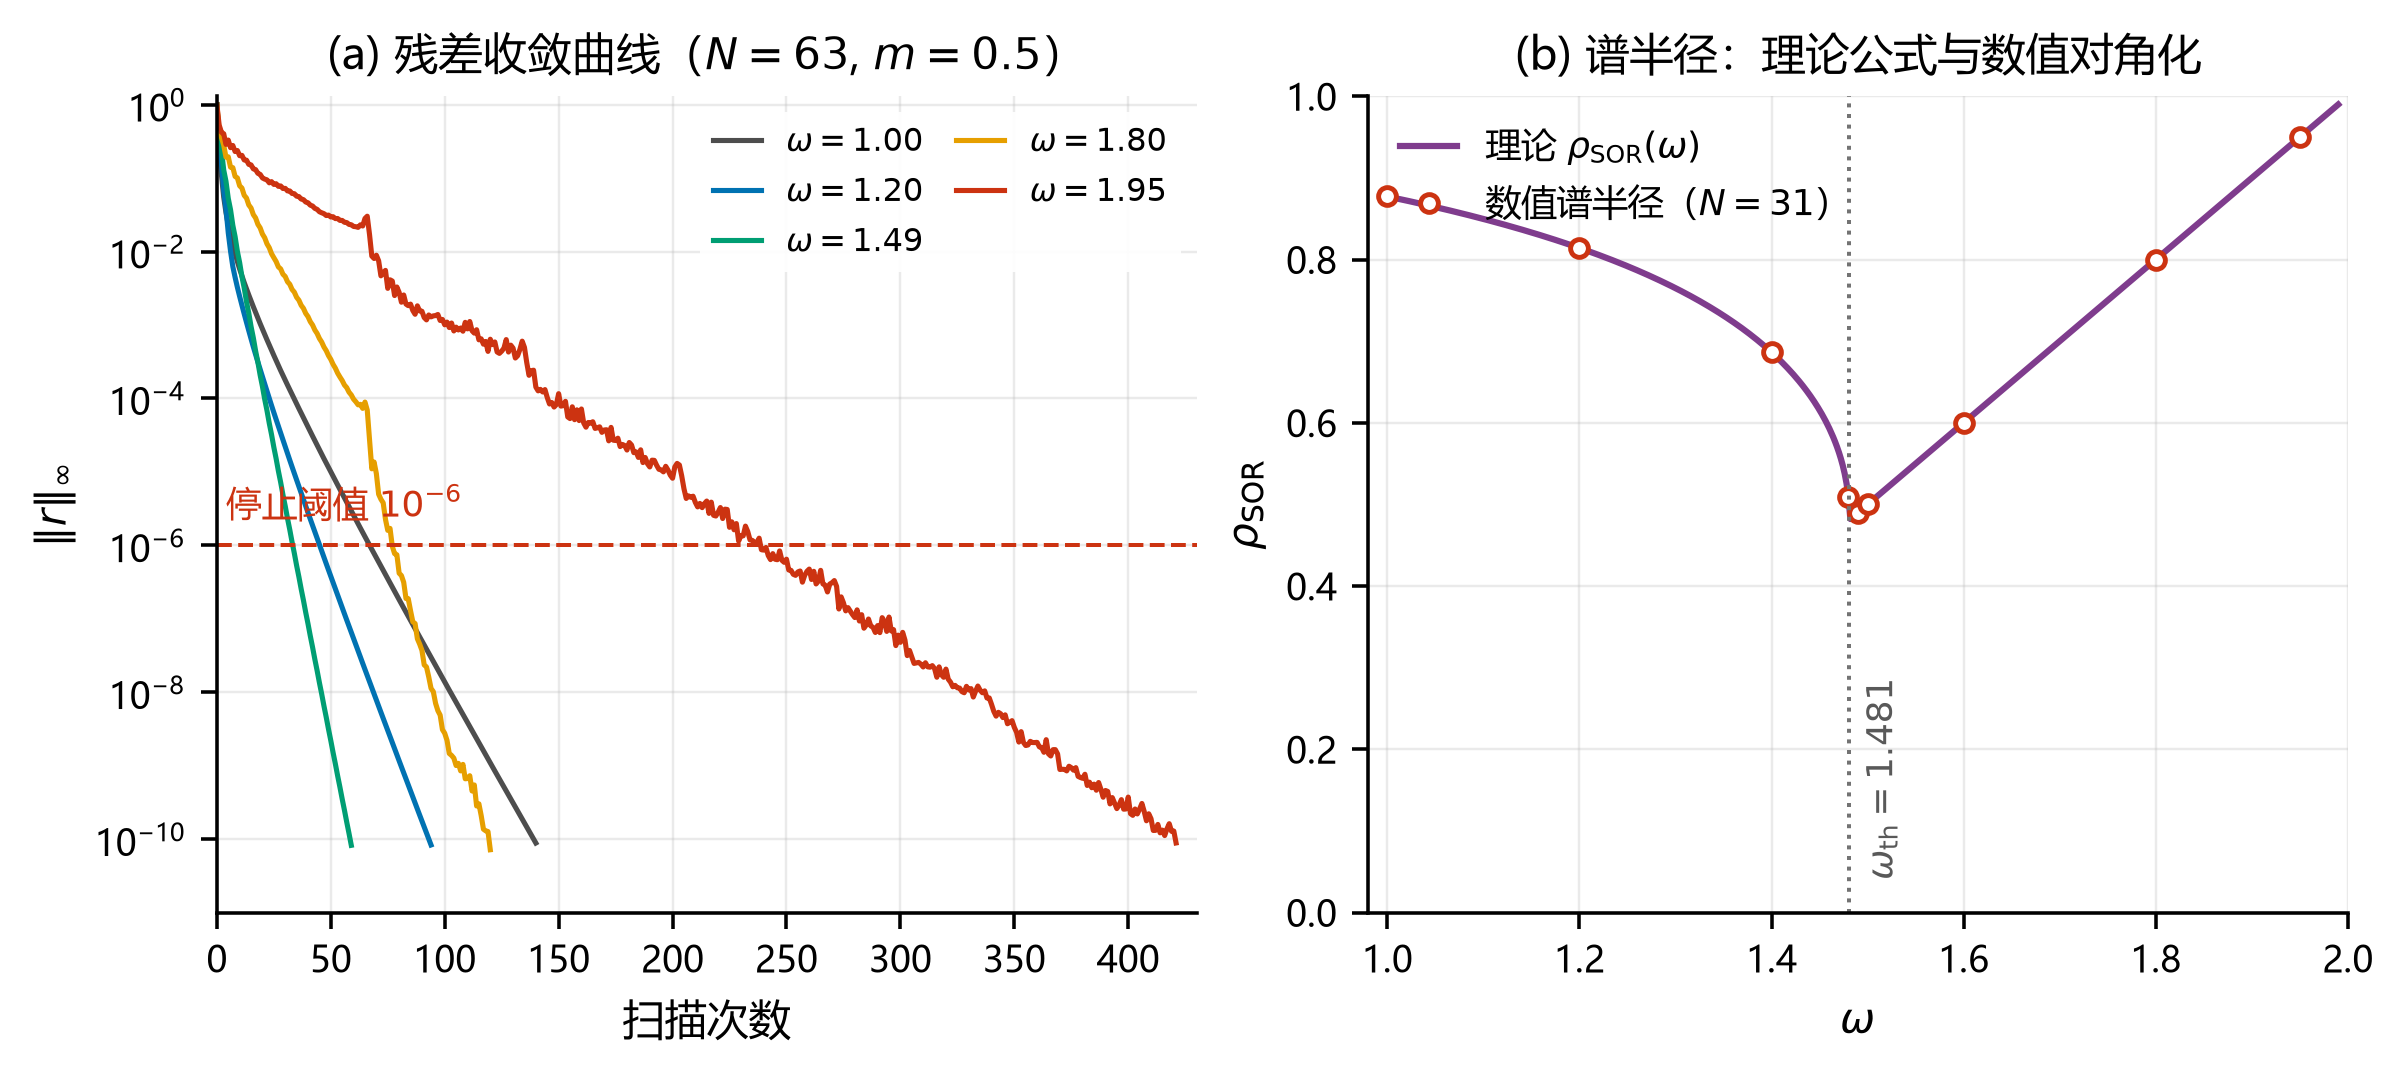
\includegraphics[width=\linewidth]{../figures/fig5_theory.png}
\caption{(a) $N=63$、$m=0.5$ 时不同 $\omega$ 的残差收敛曲线，水平虚线为正式实验的
停止阈值 $10^{-6}$；(b) $N=31$、$m=0.5$ 时 SOR 谱半径的理论公式（实线）与数值
对角化（空心圆点）。}
\label{fig:theory}
\end{figure}

\subsection{经验值与理论值的系统比较}

表~\ref{tab:theory} 把第~\ref{sec:task4} 节的实验值与式~\eqref{eq:wth}、
\eqref{eq:kasym} 的理论值放在一起。可以看到两个系统性的差异：
\begin{enumerate}[leftmargin=2.1em,itemsep=0.15em,topsep=0.2em]
\item 经验最优 $\omega$ 比 $\omega_{\rm th}$ 低 $0.057$--$0.075$；
\item 实际 $K_{\rm SOR}$ 约为 $K_{\rm SOR}^{\rm asym}$ 的 $1.36$--$1.72$ 倍，而实际
$K_{\rm GS}$ 约为 $K_{\rm GS}^{\rm asym}$ 的 $0.51$--$0.74$ 倍。
\end{enumerate}
第 2 条正好解释第 1 条：在有限阈值下，Gauss--Seidel 因初始高频被快速压低而“占便宜”，
SOR 在 $\omega_{\rm th}$ 附近因瞬态长而“吃亏”；于是实测的 $K(\omega)$ 极小点向较小的
$\omega$ 偏移。阈值越松，偏移越大；阈值越紧，两者越接近渐近理论。表~\ref{tab:threshold}
中经验最优从 $1.41$ 移到 $1.47$，就是这一机制的直接证据。

\begin{table}[htbp]
\centering
\caption{$N=63$ 时实验值与渐近理论值的比较。$K^{\rm asym}$ 由
式~\eqref{eq:kasym} 计算（$\epsilon=10^{-6}$）；$S_{\rm exp}=K_{\rm GS}/K_{\rm SOR}$，
$S_{\rm th}=K_{\rm GS}^{\rm asym}/K_{\rm SOR}^{\rm asym}$。}
\label{tab:theory}
\small
\begin{tabular}{lccc}
\toprule
量 & $m=0.2$ & $m=0.5$ & $m=1.0$ \\
\midrule
$\rho_J$ & 0.9889 & 0.9400 & 0.7990 \\
$\omega_{\rm th}$ & 1.7413 & 1.4914 & 1.2490 \\
$\omega_{\rm exp}$ & 1.684 & 1.418 & 1.174 \\
$\Delta\omega=\omega_{\rm th}-\omega_{\rm exp}$ & 0.057 & 0.073 & 0.075 \\
$K_{\rm SOR}$ & 63 & 30 & 17 \\
$K_{\rm SOR}^{\rm asym}$ & 46.2 & 19.4 & 9.9 \\
$K_{\rm GS}$ & 316 & 68 & 23 \\
$K_{\rm GS}^{\rm asym}$ & 619 & 112 & 31 \\
$S_{\rm exp}$ & 5.02 & 2.27 & 1.35 \\
$S_{\rm th}$ & 13.41 & 5.75 & 3.10 \\
\bottomrule
\end{tabular}

\end{table}

加速比的差距更值得注意：渐近理论预测 $S_{\rm th}=13.41,5.75,3.10$，而实测只有
$5.02,2.27,1.35$。这说明“SOR 比 GS 快一个量级”这类说法只适用于迭代次数很多、
渐近段很长的情形；本题 $10^{-6}$ 阈值下，$m=1.0$ 的 GS 本身只要 23 次，SOR 再快也
只能到 17 次，$S=1.35$。因此在报告加速比时，必须同时说明阈值、初值、网格和残差定义；
脱离这些条件的“加速比”没有可比性。

\subsection{关于“最佳 \texorpdfstring{$\omega$}{omega}”的解释}

综合以上结果，可以对题目中的“最佳 $\omega$”给出一个分层的回答：
\begin{itemize}[leftmargin=2.1em,itemsep=0.15em,topsep=0.2em]
\item \textbf{渐近意义下}，$\omega_{\rm th}=2/(1+\sqrt{1-\rho_J^2})$ 使谱半径最小，
是理论上最优的松弛因子；本文的数值对角化与式~\eqref{eq:rhosor} 完全一致。
\item \textbf{有限阈值、有限步数下}，实际 $K(\omega)$ 还取决于初始误差在各模式上的
投影（前因子）和迭代矩阵的瞬态；本题的 $\delta$ 源、零初值使这一效应不可忽略，
因此经验最优低于 $\omega_{\rm th}$，且随阈值变化。
\item \textbf{数值上}，最优值是一个平台而不是一个点；平台的宽度随 $m$ 变化
（$0.006$--$0.032$）。报告“平台中点 + 平台范围 + 阈值”比报告一个孤立的最优值更诚实、
更可复核。
\end{itemize}

% ===========================================================================
\section{结论与局限}
% ===========================================================================

\subsection{主要结论}

\begin{enumerate}[leftmargin=2.1em,itemsep=0.18em,topsep=0.2em]
\item 逐点 SOR 程序通过了小网格直接解对照：$N=7,9$ 上 $\epsilon_\infty$ 随阈值从
$2.3\times10^{-5}$ 单调降到 $1.1\times10^{-11}$，且满足
$\epsilon_\infty\le\|A^{-1}\|_\infty\|r\|_\infty$；转置对称性达到机器精度，正性与
最大值原理成立。
\item $N=31$、$m=0.5$、$\omega=1.5$ 的基准解在源点取最大值
$u_{\max}=\UmaxTaskI$，离开源点后先陡降、后指数衰减；$\|r\|_\infty=\RestaskI$，
共 \KtaskI{} 次扫描。
\item $N=63$ 时，$m=0.2,0.5,1.0$ 的尾段衰减长度为
$\xi=\XiA,\XiB,\XiC$，$m\xi$ 近似常数，支持 $\xi\propto1/m$。题目建议的
$r_{1/e}$ 指标被源点自能主导（$2,2,1$），不适合作为范围度量；$r_{1\%}$ 与 $\xi$
能清楚区分三种 $m$。
\item 边界条件对 $N=63$、$m\ge0.2$ 的中心区影响很小（相对差
$\le\BndA$）；$m=0.2$ 时 $\xi$ 有约 $0.65\%$ 的边界偏差，方向是使表观范围偏小。
\item $N=63$、$m=0.5$ 时，$K(\omega)$ 在 $\omega\approx1.41$--$1.43$ 形成宽平台
（$K=30$），比 Gauss--Seidel 的 68 次减少 \RedThree；$\omega\to2$ 时
$K\sim1/\ln[1/(\omega-1)]$ 发散，$\omega=1.95$ 已达 239 次。
\item 三种 $m$ 的经验最优为 $\WexpA,\WexpB,\WexpC$，理论值为
$\WthA,\WthB,\WthC$；经验值偏低 $0.06$--$0.08$，但随 $m$ 的变化趋势与理论一致。
把阈值从 $10^{-6}$ 收紧到 $10^{-12}$，经验最优从 $1.41$ 移到 $1.47$，说明差异来自
有限阈值下的瞬态/前因子，而非公式或程序错误。
\item 实测加速比 $S=5.02,2.27,1.35$ 明显小于渐近理论值 $13.41,5.75,3.10$；
阈值越松、$m$ 越大，差距越大。报告加速比时必须同时给出阈值与问题参数。
\end{enumerate}

\subsection{局限与讨论}

\begin{itemize}[leftmargin=2.1em,itemsep=0.15em,topsep=0.2em]
\item \textbf{模型局限。}本文是二维标量模型，不是格点 QCD：没有规范场、费米子、
手征对称性，也没有连续极限。$m$ 是屏蔽参数，$u$ 是经典标量场；结论只适用于这类
“格点上的 screened Poisson 方程”，不能直接搬到 QCD。
\item \textbf{几何与离散化。}理论公式 \eqref{eq:rhoj}--\eqref{eq:wth} 依赖方形网格、
五点格式和零 Dirichlet 边界；改变网格、边界或差分格式后，$\rho_J$ 与
$\omega_{\rm th}$ 都会改变。
\item \textbf{阈值与范数。}停止准则是 $\|r\|_\infty<10^{-6}$，不是误差准则；解误差
还取决于 $A^{-1}$。若改用 $L_2$ 残差或误差准则，$K$ 与经验最优都会变化。
\item \textbf{扫描分辨率。}“最优 $\omega$”是一个平台；本文用平台中点作为代表值，
并给出平台范围。更细的扫描不会改变平台，只会让边界更精确。
\item \textbf{计时。}本文只比较扫描次数，没有比较运行时间。若报告时间，需要说明
实现语言、向量化方式、硬件与计时方法；扫描次数是可移植的公平指标。
\item \textbf{精度。}全部计算为 float64；阈值最紧到 $10^{-12}$ 时，舍入误差开始
影响残差曲线的末端，但对 $10^{-6}$ 的正式结果没有影响。
\end{itemize}

% ===========================================================================
\appendix
\section{复现说明}
\label{app:repro}
% ===========================================================================

{\small

\paragraph{文件清单。}
\begin{itemize}[leftmargin=2.1em,itemsep=0.1em,topsep=0.2em]
\item \texttt{code/sor2d.py}：求解器与理论量；
\item \texttt{code/experiments.py}：全部数值实验；结果写入 \texttt{results/}（JSON、CSV 与数组文件）。
\item \texttt{code/\allowbreak plot\_figures.py}：生成 \texttt{figures/fig1}--\texttt{fig6}；
\item \texttt{code/\allowbreak make\_report\_assets.py}：生成 \texttt{report/\allowbreak numbers.tex} 与
\texttt{report/\allowbreak tab\_*.tex}；
\item \texttt{report/main.tex}：本报告源文件。
\end{itemize}

\paragraph{运行命令。}
\begin{verbatim}
python code/experiments.py
python code/plot_figures.py
python code/make_report_assets.py
cd report
xelatex main.tex
xelatex main.tex
\end{verbatim}

\paragraph{确定性与环境。}
程序不含随机数；所有参数、网格、初值、扫描顺序在代码中固定。实验环境为
Python 3.14.7、NumPy 2.5.3、Matplotlib 3.11.2；完整实验约 \Elapsed{} 秒
（不含绘图与排版）。表格中的数字由 \texttt{make\_report\_assets.py} 从
\texttt{results.json} 自动生成，避免手工抄写误差。
}

% ===========================================================================
\section{评分标准对照}
\label{app:rubric}
% ===========================================================================

\begin{table}[htbp]
\centering
\caption{评分项目与本报告对应位置的对照。}
\label{tab:rubric}
\small
\begin{tabular}{p{3.5cm}p{1.1cm}p{9.7cm}}
\toprule
评分项目 & 分值 & 本报告对应内容 \\
\midrule
模型与算法说明 & 15 & 第 1 节：式~\eqref{eq:bc}--\eqref{eq:sor} 给出边界、源、方程、
SOR 更新；式~\eqref{eq:residual}--\eqref{eq:stop} 给出残差与停止准则；
表~\ref{tab:protocol} 给出公平比较协议。 \\
程序实现与验证 & 20 & 第 2 节：反对角线与字典序等价性；朴素实现逐位对照；
表~\ref{tab:verify} 与图~\ref{fig:verify} 给出 $N=7,9$ 直接解对照、误差上界与
对称性检查；附录~\ref{app:repro} 给出复现命令。 \\
响应与 $m$ 的分析 & 15 & 第 3--4 节：图~\ref{fig:task1}、图~\ref{fig:task2}；
表~\ref{tab:task2} 给出 $r_{1/e}$、$r_{1\%}$、$\xi$ 三种指标及其定义；
表~\ref{tab:boundary} 定量评估边界影响。 \\
$\omega$ 参数扫描 & 25 & 第 5--6 节：表~\ref{tab:task3} 的粗扫、图~\ref{fig:task3}
的细扫与平台、表~\ref{tab:task4} 的三种 $m$ 对照；统一阈值 $10^{-6}$，
报告 $K_{\rm GS}$ 与 $S$。 \\
收敛行为与理论联系 & 20 & 第 7 节：图~\ref{fig:theory} 的残差曲线与谱半径核对；
式~\eqref{eq:rhoj}--\eqref{eq:kasym}；表~\ref{tab:threshold}、表~\ref{tab:rho}、
表~\ref{tab:theory}；解释经验最优低于理论值的原因。 \\
报告质量 & 5 & 全文图表均有编号、坐标轴与图例；结论与数据一致；第 8.2 节明确
说明模型局限（非 QCD、二维标量、特定离散格式）。 \\
\bottomrule
\end{tabular}
\end{table}

\noindent\textbf{自检。}所有必做任务（任务 1--4）与选做任务 5 均已完成；每个数值结论
都能在表或图中找到对应数据；所有比较均在表~\ref{tab:protocol} 的统一条件下进行；
代码可直接运行并复现全部数字。

% ===========================================================================
\begin{thebibliography}{9}
\addcontentsline{toc}{section}{参考文献}
\small
\setlength{\itemsep}{1pt}

\bibitem{handout}
课程作业说明：《研究型作业：二维格点点源模型中的 SOR 方法》，2026 年。

\bibitem{young}
D. M. Young,
\emph{Iterative Solution of Large Linear Systems},
Academic Press, 1971.

\bibitem{varga}
R. S. Varga,
\emph{Matrix Iterative Analysis}, 2nd ed.,
Springer, 2000.

\bibitem{press}
W. H. Press, S. A. Teukolsky, W. T. Vetterling, B. P. Flannery,
\emph{Numerical Recipes: The Art of Scientific Computing}, 3rd ed.,
Cambridge Univ. Press, 2007.

\bibitem{giordano}
N. J. Giordano, H. Nakanishi,
\emph{Computational Physics}, 2nd ed.,
Pearson, 2006.

\end{thebibliography}

\end{document}
